\documentclass[12pt]{article}

% ── Page layout ──────────────────────────────────────────────
\usepackage[margin=1in]{geometry}
\usepackage{setspace}
\onehalfspacing
\usepackage[mathlines]{lineno}
\linenumbers

% ── Mathematics ──────────────────────────────────────────────
\usepackage{amsmath,amssymb,amsthm}
\usepackage{mathtools}

% ── Tables and figures ───────────────────────────────────────
\usepackage{booktabs}
\usepackage{longtable}
\usepackage{array}
\usepackage{graphicx}
\usepackage{caption}
\captionsetup{font=small}

% ── Lists ────────────────────────────────────────────────────
\usepackage{enumitem}

% ── Algorithms ───────────────────────────────────────────────
\usepackage{algorithm}
\usepackage{algorithmic}

% ── Colors and links ─────────────────────────────────────────
\usepackage{xcolor}
\usepackage[colorlinks=true,linkcolor=blue,citecolor=blue,urlcolor=blue]{hyperref}

% ── Bibliography ─────────────────────────────────────────────
\usepackage[numbers,sort&compress]{natbib}

% ── Theorem environments ─────────────────────────────────────
\newtheorem{theorem}{Theorem}
\newtheorem{proposition}[theorem]{Proposition}
\newtheorem{lemma}[theorem]{Lemma}
\newtheorem{corollary}[theorem]{Corollary}
\newtheorem{definition}[theorem]{Definition}
\newtheorem{remark}[theorem]{Remark}
\newtheorem{example}[theorem]{Example}

% ── Line-breaking tolerance ──────────────────────────────────
\emergencystretch=1em

% ── Custom operators ─────────────────────────────────────────
\DeclareMathOperator{\TIP}{TIP}
\DeclareMathOperator{\supp}{supp}
\DeclareMathOperator{\Rips}{Rips}
\DeclareMathOperator{\diam}{diam}
\DeclareMathOperator{\Tr}{Tr}
\DeclareMathOperator*{\argmin}{arg\,min}

\title{CC-SPR: Geometry-Sensitive Sparse Persistent Representatives\\
for Interpretable Omics Feature Selection\\[6pt]
\large A Cross-Domain Evaluation Across Cancer and Plant Transcriptomics}

% PLACEHOLDER: Replace with actual author names and affiliations
\author{
  Author One$^{1,\ast}$ \and
  Author Two$^{1}$ \and
  Author Three$^{1}$\\[6pt]
  \small $^{1}$[Department], [Institution], [City], [Country]\\
  \small $^\ast$Corresponding author: \href{mailto:author@institution.edu}{author@institution.edu}
}

\date{}

\begin{document}
\maketitle

% ============================================================
%  ABSTRACT — Structured (Bioinformatics style)
% ============================================================
\begin{abstract}
\noindent\textbf{Motivation:}
Harmonic persistent homology bridges topology and biology by associating
representative cycles with molecular features, but uses dense $\ell_2$
representatives and a fixed Euclidean metric---limiting interpretability and
adaptability to the geometric heterogeneity of omics data.

\noindent\textbf{Results:}
We introduce \textbf{CC-SPR} (Cycle-Consistent Sparse Persistent
Representatives), which replaces the dense harmonic objective with a convex
elastic-net formulation and lifts the sample-space metric to a selectable
\emph{backend} family (Euclidean, Ollivier--Ricci, diffusion, PHATE-like,
and distance-to-measure).
All five backends are benchmarked on three cancer-genomics datasets
(TCGA-LUAD, GSE161711, GSE165087) and a plant developmental atlas
(Arabidopsis root, GSE123013).
Backend ranking is dataset-dependent: DTM leads on pilot LUAD ($n{=}60$,
F1${=}0.5315$); Ricci leads at full scale ($n{=}275$, F1${=}0.6339$); Euclidean
leads on GSE161711 (F1${=}0.7483$).
Zero genes are shared across all six backend configurations on LUAD, and
DTM uniquely recovers xenobiotic metabolism via cytochrome P450
(KEGG; adj.\ $p = 7{\times}10^{-4}$).
CC-SPR representatives are 2.8$\times$ sparser than harmonic representatives
while preserving comparable clustering structure.

\noindent\textbf{Availability and implementation:}
Source code, experiment scripts, and reproduction instructions are available
at \url{https://github.com/ChimdiWalter/Omics_Project_CCSPR}.

\noindent\textbf{Contact:} \href{mailto:author@institution.edu}{author@institution.edu}

\noindent\textbf{Supplementary information:} Supplementary data are available at
\textit{Bioinformatics} online.
\end{abstract}

\noindent\textbf{Keywords:} topological data analysis, persistent homology,
omics feature selection, geometry-aware, sparse optimization

\newpage

% ============================================================
% 1  INTRODUCTION
% ============================================================
\section{Introduction}
\label{sec:introduction}

\subsection{Biological motivation}

Modern omics experiments---bulk RNA-seq, single-cell transcriptomics, methylation arrays, proteomics---routinely produce data matrices with $n$ samples in $10^1$--$10^5$ and $p$ features in $10^3$--$10^5$.
These matrices encode geometry that reflects biological structure:
tumor subtypes form clusters; differentiation trajectories trace manifold-like paths; regulatory circuits create loop-like patterns in expression space; and microenvironment heterogeneity introduces curvature and density variation.
This geometric richness makes omics a natural setting for topological data analysis (TDA) \cite{carlsson2009, edelsbrunner2010}, which has been applied to gene expression landscapes \cite{rizvi2017}, protein structure \cite{xia2014}, tumor microenvironments \cite{vipond2021}, single-cell trajectories \cite{moon2019phate}, neural population coding \cite{giusti2015}, and viral evolution \cite{chan2013topology}.

Persistent homology, the workhorse of TDA, captures collective structure---loops, voids, connected components---that cannot be detected by feature-wise statistics or pairwise correlations alone.
However, the standard pipeline has a well-known interpretability gap: while a barcode tells us \emph{that} a topological feature exists and \emph{how long} it persists, it does not tell us \emph{which samples} participate in the corresponding cycle, nor \emph{which molecular features} drive it.

\subsection{The harmonic PH advance and its limitations}

Harmonic persistent homology \cite{harmonicPH} addresses this gap by computing a representative cycle for each persistent class that minimizes an $\ell_2$ (harmonic) energy, creating a bridge from topological features back to individual samples and molecular features.
However, two practical limitations motivate the present work:
\begin{enumerate}[leftmargin=1.5em]
\item \textbf{Dense representatives blur interpretation.}
The harmonic $\ell_2$ objective spreads weight broadly across edge support.
In omics, where the goal is to identify compact gene sets associated with topological signals, dense support complicates downstream pathway analysis.
\item \textbf{Euclidean geometry may be inappropriate.}
The default sample-space metric is Euclidean distance, which is often too rigid for biological data with nonuniform density, curvature-rich manifold structure, or developmental trajectories.
Different metrics can produce different filtrations and different representatives---a sensitivity that should be modeled explicitly.
\end{enumerate}

\subsection{Contributions}

We introduce \textbf{CC-SPR} (Cycle-Consistent Sparse Persistent Representatives), which addresses both limitations within the harmonic persistent homology scaffold:
\begin{enumerate}[leftmargin=1.5em]
\item \textbf{Sparse elastic representatives.} We replace the dense $\ell_2$ objective with a convex elastic-net objective that concentrates cycle support on a small number of edges, yielding interpretable, bootstrap-stable feature-importance profiles.
\item \textbf{Backend-aware geometry.} We formalize the sample-space metric as a selectable backend, implementing Euclidean, Ollivier--Ricci, diffusion, PHATE-like, and distance-to-measure (DTM) geometry families.
\item \textbf{Topological influence profiles (TIP).} We introduce a bootstrap-aggregated feature-stability diagnostic that enables direct comparison of support concentration across geometries.
\item \textbf{Cross-domain evaluation.} We benchmark all five backends on three cancer-genomics datasets and provide targeted cross-domain evidence on plant transcriptomics.
\end{enumerate}

CC-SPR is not a claim of predictive superiority over standard classifiers.
It is a framework that makes topology-derived features more interpretable and geometry-aware; every harmonic PH analysis is a special case with $\lambda_1 = 0$ and a Euclidean backend.


% ============================================================
% 2  MATERIALS AND METHODS
% ============================================================
\section{Materials and Methods}
\label{sec:methods}

% ── 2.1 Datasets ─────────────────────────────────────────────
\subsection{Datasets}
\label{sec:datasets}

We use four datasets with distinct evaluation roles (Table~\ref{tab:datasets}):
\begin{itemize}[leftmargin=1.5em]
\item \textbf{TCGA-LUAD} (lung adenocarcinoma, $p \approx 20{,}000$): main benchmark anchor.
Evaluated at two scales: pilot ($n = 60$, 2-split CV, $n_{\text{boot}} = 5$) and full cohort ($n = 275$, 5-fold CV, $n_{\text{boot}} = 5$, 2000 variable genes).
\item \textbf{GSE161711} (CLL/venetoclax bulk RNA-seq, $n = 96$): disease-aligned bulk validation with 5-fold CV.
\item \textbf{GSE165087} (CLL/RS-like scRNA-seq, bounded $n = 320$): bounded single-cell feasibility test with all five backends.
\item \textbf{Arabidopsis root atlas} (GSE123013 \cite{denyer2019}, scRNA-seq, $n = 500$, 16 Leiden clusters): targeted cross-domain generalization test with Euclidean and DTM only.
\end{itemize}

\begin{table}[h]
\centering\small
\begin{tabular}{llccl}
\toprule
Dataset & Type & $n$ & $p$ & Labels \\
\midrule
TCGA-LUAD (pilot) & Bulk RNA-seq & 60 & 20,530 & Molecular subtype \\
TCGA-LUAD (full) & Bulk RNA-seq & 275 & 20,530 & Molecular subtype \\
GSE161711 & Bulk RNA-seq & 96 & 17,860 & Venetoclax response \\
GSE165087 & scRNA-seq & 320 & 5,000 & CLL vs Richter \\
Arabidopsis root & scRNA-seq & 500 & 21,965 & Leiden cluster (16 types) \\
\bottomrule
\end{tabular}
\caption{Datasets used in this study. GSE161711 and GSE165087 are public GEO substitutes for originally intended controlled-access datasets.}
\label{tab:datasets}
\end{table}

% ── 2.2 The CC-SPR framework ─────────────────────────────────
\subsection{The CC-SPR framework}
\label{sec:ccspr_framework}

CC-SPR preserves the four-step harmonic persistent homology scaffold---construct a sample-space metric, compute a filtration and persistent homology, choose a representative cycle, project to feature space---but modifies two steps: the representative objective (Step~3) and the metric (Step~1).

\paragraph{Notation.}
Let $X \in \mathbb{R}^{n \times p}$ denote an omics data matrix.
A \emph{geometry backend} $\mathcal{G}$ with hyperparameters $\theta_{\mathcal{G}}$ induces a symmetric distance matrix $D^{(\mathcal{G})} \in \mathbb{R}_{\ge 0}^{n \times n}$.
The Vietoris--Rips filtration on $D^{(\mathcal{G})}$ produces a nested sequence of simplicial complexes whose homology yields a persistence barcode $\{[b_i, d_i)\}$ \cite{zomorodian2005, edelsbrunner2010}.
We focus on $H_1$ bars because 1-cycles in sample space project to feature space via the data matrix, creating a bridge from topological structure to gene-level influence.

\paragraph{Harmonic (dense) objective.}
For a selected $H_1$ bar $[b, d)$ with initial cycle $z_0 \in C_1$ and boundary operator $\partial_2$, the harmonic representative minimizes
\begin{equation}\label{eq:harmonic}
\hat{y}_{\mathrm{harm}} = \argmin_{y \in C_2} \| z_0 + \partial_2 y \|_2^2.
\end{equation}
This produces the smoothest cycle, typically with dense edge support ($\|z\|_0 = O(|E|)$), which dilutes biological signal when projected to feature space \cite{harmonicPH, friedman1998}.

\paragraph{Sparse elastic objective.}
CC-SPR replaces (\ref{eq:harmonic}) with an elastic-net formulation:
\begin{equation}\label{eq:ccspr}
\hat{y}_{\mathrm{spr}} = \argmin_{y \in C_2} \;\underbrace{\| z_0 + \partial_2 y \|_2^2}_{\text{fidelity}} + \underbrace{\lambda_1 \| z_0 + \partial_2 y \|_1}_{\text{sparsity}} + \underbrace{\lambda_2 \| y \|_2^2}_{\text{stability}},
\end{equation}
with $\lambda_1, \lambda_2 \ge 0$.
The objective is convex (strongly convex when $\lambda_2 > 0$), and the $\ell_1$ penalty drives small edge weights to zero, producing representatives with compact support (see Supplementary Section~S2 for proofs of convexity and sparsity guarantees).
The structure mirrors the elastic net \cite{zou2005elasticnet}: $\lambda_1$ plays the LASSO role promoting sparsity, $\lambda_2$ provides ridge-like stability, and the ``design matrix'' is the boundary operator $\partial_2$.

% ── 2.3 Topological influence profiles ────────────────────────
\subsection{Topological influence profiles (TIP)}
\label{sec:tip}

For bootstrap replicates $b = 1, \ldots, B$ and a top-$K$ feature selection threshold, let $S_b$ denote the set of features with the $K$ largest absolute projected weights from the sparse representative in replicate $b$.
The \emph{topological influence profile} is
\[
\TIP(j) = \frac{1}{B} \sum_{b=1}^B \mathbf{1}\{j \in S_b\}, \qquad j = 1, \ldots, p.
\]
Concentrated TIP mass (a few features with $\TIP(j) \approx 1$) indicates stable topological signal; diffuse mass indicates unstable support.
Because TIP applies identically to any geometry backend, it provides a natural diagnostic for comparing how backends affect interpretability.

% ── 2.4 Geometry backends ─────────────────────────────────────
\subsection{Geometry backends}
\label{sec:backends}

A central design principle of CC-SPR is that the sample-space metric is a selectable parameter, not a fixed assumption.
Backend choice can be understood as a controlled perturbation: when the distance matrices from two backends differ by $\varepsilon_\infty$ in the $\ell_\infty$ norm, the bottleneck distance between persistence diagrams is bounded by $\varepsilon_\infty$ \cite{chazal2014persistence}.
We implement five backends:

\paragraph{Euclidean (baseline).}
Standard $\ell_2$ distance in PCA space: $D^{(\text{eu})}_{ij} = \|x_i - x_j\|_2$.
Simple and efficient, but rigid---it treats all directions equally and does not adapt to local density or curvature.

\paragraph{Ollivier--Ricci curvature.}
The Ollivier--Ricci curvature \cite{ollivier2007,ollivier2009} of an edge $(u,v)$ is $\kappa(u,v) = 1 - W_1(\mu_u, \mu_v)/d(u,v)$, where $W_1$ is the Wasserstein-1 distance between neighborhood measures.
Discrete Ricci flow \cite{ni2019community} iteratively updates edge weights: $w_{uv}^{(t+1)} = w_{uv}^{(t)} - \eta \cdot \kappa^{(t)}(u,v) \cdot w_{uv}^{(t)}$, upweighting negatively curved (bridge) edges.
This delays merger of distinct components in the filtration, potentially preserving genuine cycles at the expense of noise-induced shortcuts.

\paragraph{Diffusion.}
Diffusion distances \cite{coifman2006diffusion} are derived from the eigendecomposition of a Markov transition matrix $P = D_W^{-1}W$, capturing connectivity that persists across random walks of varying length.
A time parameter $t$ controls scale: small $t$ recovers local geometry; large $t$ emphasizes global connectivity.
Implemented via truncated eigendecomposition (50 eigenvectors).

\paragraph{PHATE-like.}
PHATE \cite{moon2019phate} transforms diffusion operators via a log potential: $U_i = -\log(P^t_{i,\cdot} + \epsilon)$, with potential distance $D^{(\text{phate})}(i,j) = \|U_i - U_j\|_2$.
This measures how differently random walks from $i$ and $j$ explore the graph, approximating a Fisher--Rao-like distance.
Our implementation uses a lightweight potential-distance computation without the full MDS step.

\paragraph{Distance-to-measure (DTM).}
DTM \cite{chazal2011dtm, chazal2017robust} replaces pairwise distances with density-smoothed variants: $d_{\mu_X, m_0}(x) = (\frac{1}{\lceil m_0 n \rceil} \sum_{j=1}^{\lceil m_0 n \rceil} \|x - x_{(j)}\|^2)^{1/2}$.
DTM-weighted distances delay inclusion of outlier-adjacent simplices, suppressing topological noise from density spikes---relevant for omics data with batch effects, dropout, or technical outliers.

% ── 2.5 Evaluation protocol ──────────────────────────────────
\subsection{Evaluation protocol}
\label{sec:evaluation}

All five backends are evaluated under the same pipeline: backend $\to$ Rips filtration $\to$ persistent homology $\to$ sparse representative $\to$ TIP $\to$ feature selection $\to$ weighted-F1 classification (logistic regression).
Dataset-appropriate replication:
\begin{itemize}[leftmargin=1.5em]
\item LUAD pilot: 2-split CV, $n_{\text{boot}} = 5$; all five backends.
\item LUAD full: 5-fold CV, $n_{\text{boot}} = 5$, 2000 variable genes; all five backends.
\item GSE161711: 5-fold CV, $n_{\text{boot}} = 5$; all five backends.
\item GSE165087: 1 split, $n_{\text{boot}} = 1$; all five backends.
\item Arabidopsis: 3-fold CV, $n_{\text{boot}} = 3$; Euclidean and DTM only.
\end{itemize}

\paragraph{Leakage control.}
Within each training fold: (1)~variable genes are selected by variance on training data only; (2)~standardization uses training-derived parameters; (3)~bootstrap TIP computation uses training-fold subsamples only; (4)~feature selection and classifier training operate exclusively on training data.
Two departures from a fully strict within-fold protocol: global PCA where applied (single-cell data), and full-dataset variable-gene selection in the standard baseline only at full LUAD scale.
Both are documented and apply identically across all methods.

\paragraph{Resource policy.}
Experiments were conducted in two phases: Phase~1 on an HPC cluster (48\,GB, 8 CPUs; pilot LUAD, GSE161711, GSE165087) and Phase~2 on a local workstation (Intel i9-9920X, 24 threads, 125\,GB RAM; full-scale LUAD and Arabidopsis).
Rather than silently omitting failed runs, completed outputs are reused and resource limits are stated explicitly.

% ── 2.6 Pipeline algorithm ────────────────────────────────────
\subsection{Pipeline algorithm}
\label{sec:algorithm}

\begin{algorithm}[h]
\caption{CC-SPR Pipeline}
\label{alg:ccspr}
\begin{algorithmic}[1]
\REQUIRE Data matrix $X \in \mathbb{R}^{n \times p}$, geometry backend $\mathcal{G}$, parameters $\lambda_1, \lambda_2, k, K$, bootstraps $B$
\ENSURE Topological influence profile $\TIP \in [0,1]^p$
\STATE Compute distance matrix $D^{(\mathcal{G})} \gets \texttt{Backend}(X, \mathcal{G})$
\STATE Compute Vietoris--Rips filtration and persistent homology on $D^{(\mathcal{G})}$
\STATE Select the most persistent $H_1$ bar $[b, d)$
\STATE Extract initial cycle $z_0$ and boundary operator $\partial_2$ at scale $\varepsilon = (b + d)/2$
\FOR{$b = 1, \ldots, B$}
    \STATE Draw bootstrap resample $X^{(b)}$ of size $n$
    \STATE Recompute $D^{(\mathcal{G})(b)}$, filtration, and persistent homology
    \STATE Solve \eqref{eq:ccspr} to obtain $\hat{z}_{\mathrm{spr}}^{(b)}$
    \STATE Project $\hat{z}_{\mathrm{spr}}^{(b)}$ to feature space: $w^{(b)} \in \mathbb{R}^p$
    \STATE Select top-$K$ features: $S_b \gets \{j : |w^{(b)}_j| \text{ among top-}K\}$
\ENDFOR
\STATE Compute $\TIP(j) \gets \frac{1}{B} \sum_{b=1}^B \mathbf{1}\{j \in S_b\}$ for each feature $j$
\RETURN $\TIP$
\end{algorithmic}
\end{algorithm}

\paragraph{Computational complexity.}
The dominant costs are distance matrix computation ($O(n^2 p)$ for Euclidean; higher for Ricci flow and diffusion eigendecomposition), persistent homology ($O(m^3)$ worst case, much faster in practice \cite{gudhi2014}), and sparse optimization ($O(|E|^2 \cdot |F|)$ per bootstrap).
Total cost is $O(B \cdot (n^2 p + m^3))$, dominated by the bootstrap loop.
Full-scale LUAD ($n = 275$) requires 35 minutes to 2.5 hours per backend; the CVXPY elastic-net solver on the boundary matrix is the computational bottleneck.

% ── 2.7 Comparison with harmonic PH ──────────────────────────
\subsection{Comparison with harmonic PH}
\label{sec:comparison}

Table~\ref{tab:hphcompare} provides a systematic comparison of harmonic PH and CC-SPR.

\begin{table}[h]
\centering
\small
\begin{tabular}{p{2.5cm}p{3.0cm}p{3.0cm}}
\toprule
\textbf{Axis} & \textbf{Harmonic PH} & \textbf{CC-SPR} \\
\midrule
Metric assumption & Fixed Euclidean & Selectable backend family \\
Representative criterion & Dense $\ell_2$ (harmonic) & Sparse elastic net \\
Sparsity & No explicit control & $\lambda_1$-controlled \\
Interpretability & Diffuse feature weights & Concentrated feature weights \\
Stability diagnostics & Not built-in & TIP profiles (bootstrap) \\
Computational cost & Moderate & Moderate to high (backend-dependent) \\
Backend flexibility & None (single metric) & Euclidean, Ricci, diffusion, PHATE, DTM \\
Biological alignment & Medium (diluted signal) & High (compact gene sets) \\
\bottomrule
\end{tabular}
\caption{Comparison of harmonic PH and CC-SPR. CC-SPR extends harmonic PH by adding sparsity control, stability diagnostics, and geometry awareness while preserving the same scaffold.}
\label{tab:hphcompare}
\end{table}

The harmonic representative is sufficient when cycle support is naturally compact, downstream tasks do not require feature attribution, or datasets are small enough that dense support does not dilute signal.
CC-SPR adds value when compact gene-set identification, geometry sensitivity analysis, or bootstrap stability assessment is required.

% ============================================================
% 3  RESULTS
% ============================================================
\section{Results}
\label{sec:results}

% ── 3.1 Backend ranking is dataset-dependent ──────────────────
\subsection{Backend ranking is dataset-dependent}
\label{sec:benchmark}

The central empirical question is whether the five geometry backends produce meaningfully different results across datasets.
Table~\ref{tab:geobench} presents the complete geometry-family benchmark.

\begin{table}[h]
\centering
\small
\begin{tabular}{@{}llccr@{}}
\toprule
Dataset & Backend & Mean F1 & Std F1 & $N$ splits \\
\midrule
LUAD ($n=60$) & euclidean & 0.4342 & 0.0394 & 2 \\
LUAD & ricci & 0.5012 & 0.1073 & 2 \\
LUAD & diffusion & 0.5000 & 0.1000 & 2 \\
LUAD & phate\_like & 0.3546 & 0.0880 & 2 \\
LUAD & dtm & 0.5315 & 0.0765 & 2 \\
\midrule
GSE161711 ($n=96$) & euclidean & 0.7483 & 0.0825 & 5 \\
GSE161711 & ricci & 0.5944 & 0.0845 & 5 \\
GSE161711 & diffusion & 0.5553 & 0.0721 & 5 \\
GSE161711 & phate\_like & 0.5396 & 0.0632 & 5 \\
GSE161711 & dtm & 0.6178 & 0.1333 & 5 \\
\midrule
GSE165087 (bounded, $n=320$) & all backends & 0.9254 & 0.0 & 1 \\
\midrule
Arabidopsis root ($n=500$) & euclidean & 0.5933 & 0.1660 & 3 \\
Arabidopsis root & dtm & \textbf{0.6664} & 0.0940 & 3 \\
Arabidopsis root & standard & 0.9585 & 0.0170 & 3 \\
\midrule
LUAD full ($n=275$) & euclidean & 0.5655 & 0.0361 & 5 \\
LUAD full & ricci & \textbf{0.6339} & 0.0503 & 5 \\
LUAD full & diffusion & 0.5522 & 0.0609 & 5 \\
LUAD full & phate\_like & 0.5445 & 0.0640 & 5 \\
LUAD full & dtm & 0.5814 & 0.0611 & 5 \\
LUAD full & standard & 0.7501 & 0.0294 & 5 \\
\bottomrule
\end{tabular}
\caption{Geometry-family benchmark across four datasets.
Backend ranking is dataset-dependent and scale-sensitive: on pilot LUAD, DTM $>$ Ricci $\approx$ Diffusion $>$ Euclidean $>$ PHATE-like; at full scale, Ricci overtakes DTM ($0.6339$ vs $0.5814$); on GSE161711, Euclidean $\gg$ all others.}
\label{tab:geobench}
\end{table}

On pilot LUAD, DTM leads ($0.5315$), consistent with density-aware distances better capturing heterogeneous subtype topology.
At full scale ($n = 275$), Ricci overtakes DTM ($0.6339$ vs $0.5814$), suggesting curvature correction benefits from denser point clouds.
On GSE161711, Euclidean dominates ($0.7483$, $+0.1305$ over DTM), indicating that local PCA neighborhoods suffice for this more homogeneous cohort.
All backends produce identical F1 on the resource-bounded GSE165087 configuration.

\textbf{Takeaway:} No single backend is universally best; backend ranking depends on dataset structure and sample size.

% ── 3.2 Historical context ───────────────────────────────────
\subsection{Comparison with harmonic and standard baselines}

Table~\ref{tab:baselines} provides historical context from the initial two-backend evaluation.

\begin{table}[h]
\centering
\small
\begin{tabular}{llcc}
\toprule
Dataset & Model & Mean F1 & $N$ \\
\midrule
LUAD ($n=60$) & standard & 0.7670 & 2 \\
LUAD ($n=60$) & harmonic & 0.4044 & 2 \\
LUAD ($n=60$) & ccspr (Ricci) & 0.3133 & 2 \\
\midrule
GSE161711 & standard & 0.9711 & 5 \\
GSE161711 & harmonic & 0.5850 & 5 \\
GSE161711 & ccspr (Ricci) & 0.6028 & 5 \\
\midrule
GSE165087 (bounded) & all methods & 0.9254 & 1 \\
\bottomrule
\end{tabular}
\caption{Historical baseline comparison from the initial two-backend evaluation. Standard baselines dominate on raw F1; the gap narrows from $0.236$ at pilot scale to $0.116$ at full scale.}
\label{tab:baselines}
\end{table}

Expanding the backend family and increasing sample size both improve CC-SPR performance: the original Ricci-only result (F1 $= 0.3133$) improves to DTM $= 0.5315$ at pilot scale and Ricci $= 0.6339$ at full scale.

\textbf{Takeaway:} Standard baselines remain strongest on raw F1, but the CC-SPR--standard gap narrows with scale and backend optimization.

% ── 3.3 Paired statistics ────────────────────────────────────
\subsection{LUAD multiseed paired statistics}

The multiseed analysis measures paired differences across 18 repeated splits, controlling for split-specific data variation (Table~\ref{tab:paired}).

\begin{table}[h]
\centering
\small
\begin{tabular}{lcccc}
\toprule
Comparison & $n$ & Mean $\Delta$ & Paired $t$ ($p$) & Wilcoxon ($p$) \\
\midrule
CC-SPR vs harmonic & 18 & $+0.027$ & 0.514 & 0.495 \\
CC-SPR vs standard & 18 & $-0.186$ & $2.7 \times 10^{-4}$ & $3.3 \times 10^{-4}$ \\
Ricci sparse vs Eu.\ sparse & 18 & $+0.046$ & 0.308 & 0.265 \\
\bottomrule
\end{tabular}
\caption{LUAD multiseed paired statistics ($n=18$ splits). CC-SPR significantly underperforms the standard baseline ($p < 0.001$). The Ricci advantage ($+0.046$) is substantively interesting but not significant at this sample size.}
\label{tab:paired}
\end{table}

The five-backend results corroborate the Ricci direction: Ricci exceeds Euclidean at both pilot ($+0.067$) and full scale ($+0.068$).

\begin{figure}[h]
\centering
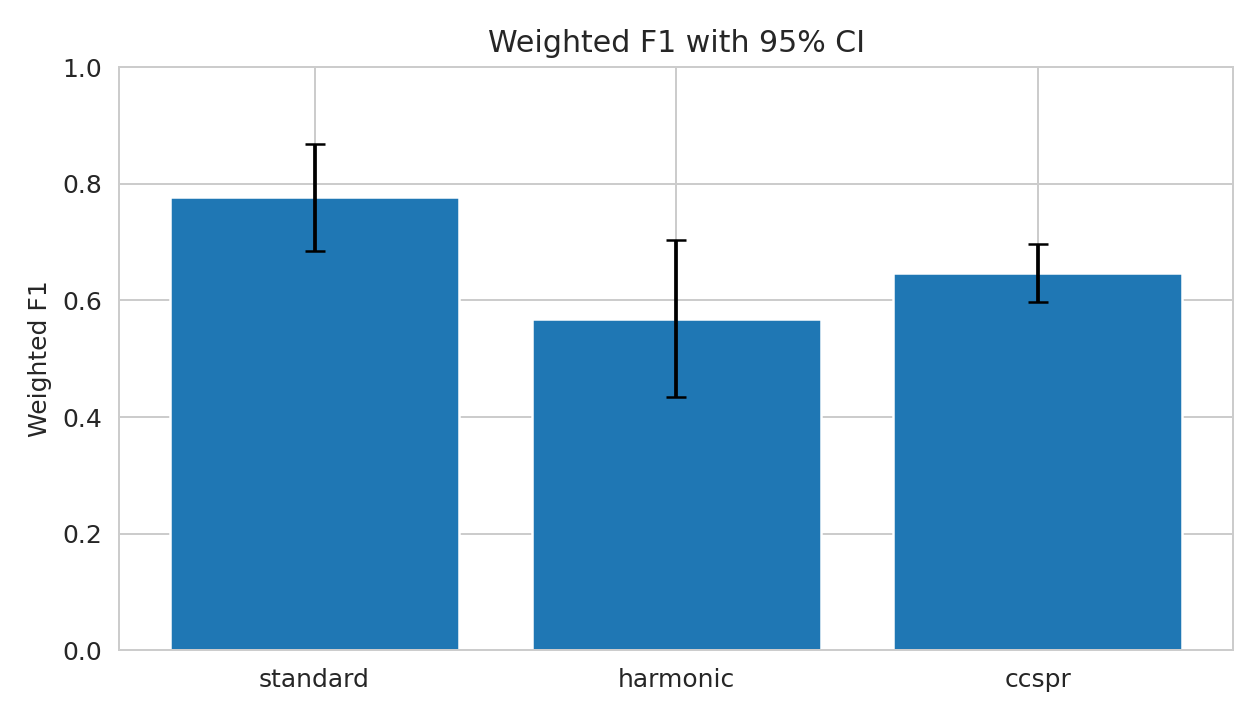
\includegraphics[width=0.49\linewidth]{figures/f1_bars_ci.png}
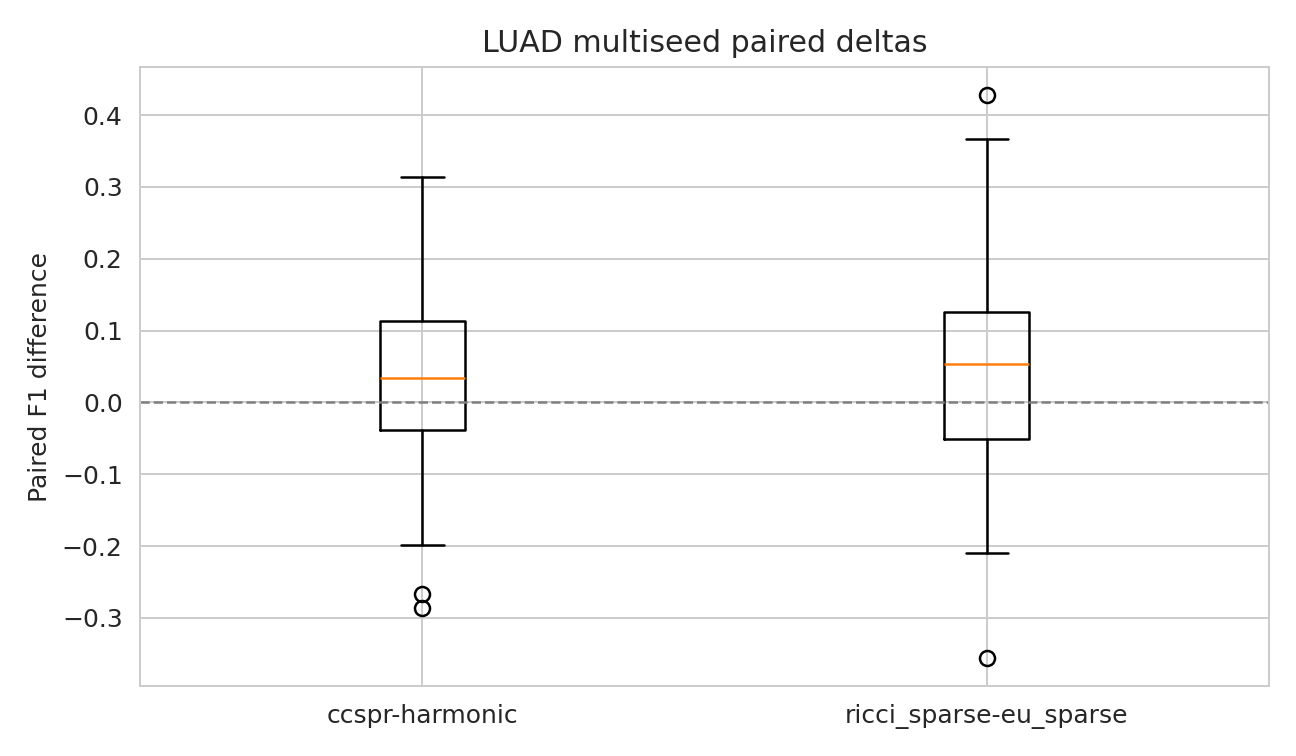
\includegraphics[width=0.49\linewidth]{figures/paired_deltas_luad_multiseed.png}
\caption{\textbf{Left}: LUAD benchmark showing the predictive gap between standard baseline and topology-derived models.
\textbf{Right}: Paired multiseed deltas across 18 splits. CC-SPR vs standard is significantly negative; Ricci vs Euclidean sparse is positive but not significant.}
\label{fig:luad}
\end{figure}

% ── 3.4 Topological diagnostics ──────────────────────────────
\subsection{Topological diagnostics across the geometry family}

Beyond classification, the five-backend evaluation provides rich topological diagnostics (Tables~\ref{tab:diag_luad} and \ref{tab:diag_gse}).

\begin{table}[h]
\centering
\small
\begin{tabular}{@{}lcccccccc@{}}
\toprule
Backend & $n_{\text{ok}}$ & $\bar{\ell}$ & $\sigma_\ell$ & $\bar{\rho}$ & $\sigma_\rho$ & Support & TIP Ent. & TIP Gini \\
\midrule
euclidean & 5 & 0.0798 & 0.0250 & 0.0469 & 0.0296 & 50 & 3.7327 & 0.3212 \\
ricci & 4 & 0.0130 & 0.0067 & 0.0067 & 0.0080 & 71 & 4.2261 & 0.0982 \\
diffusion & 5 & 0.0256 & 0.0177 & 0.0146 & 0.0145 & 78 & 4.2740 & 0.1797 \\
phate\_like & 4 & 0.0112 & 0.0100 & 0.0085 & 0.0076 & 80 & 4.3820 & 0.0000 \\
dtm & 5 & 0.0083 & 0.0059 & 0.0068 & 0.0068 & 76 & 4.2725 & 0.1642 \\
\bottomrule
\end{tabular}
\caption{LUAD topological diagnostics. Euclidean produces the highest $H_1$ lifetime ($0.0798$) and most concentrated TIP (Gini $= 0.3212$). PHATE-like produces zero Gini (uniform TIP), suggesting over-smoothing.}
\label{tab:diag_luad}
\end{table}

\begin{table}[h]
\centering
\small
\begin{tabular}{@{}lcccccccc@{}}
\toprule
Backend & $n_{\text{ok}}$ & $\bar{\ell}$ & $\sigma_\ell$ & $\bar{\rho}$ & $\sigma_\rho$ & Support & TIP Ent. & TIP Gini \\
\midrule
euclidean & 5 & 0.0828 & 0.0025 & 0.0118 & 0.0079 & 59 & 4.0106 & 0.1861 \\
ricci & 5 & 0.1248 & 0.0482 & 0.0468 & 0.0407 & 95 & 4.5359 & 0.0474 \\
diffusion & 5 & 0.0426 & 0.0235 & 0.0213 & 0.0206 & 93 & 4.5081 & 0.0647 \\
phate\_like & 5 & 0.0091 & 0.0074 & 0.0049 & 0.0050 & 84 & 4.3729 & 0.1362 \\
dtm & 5 & 0.0487 & 0.0078 & 0.0166 & 0.0059 & 24 & 3.1300 & 0.1300 \\
\bottomrule
\end{tabular}
\caption{GSE161711 topological diagnostics. Ricci produces the longest $H_1$ lifetime ($0.1248$) despite ranking third on classification. DTM produces the most compact support (24 features vs 59--95).}
\label{tab:diag_gse}
\end{table}

Key findings:
Euclidean's highest $H_1$ lifetime and TIP Gini on LUAD do not translate to the highest classification F1---concentration alone is not sufficient for downstream performance.
On GSE161711, Ricci creates the most persistent topological features ($H_1$ lifetime $= 0.1248$) but trails Euclidean on classification ($0.5944$ vs $0.7483$), illustrating that persistent topology captures structure complementary to class separation.
DTM's projected support on GSE161711 (24 features vs 59--95) demonstrates the concentration effect of outlier-robust distances.

\begin{figure}[h]
\centering
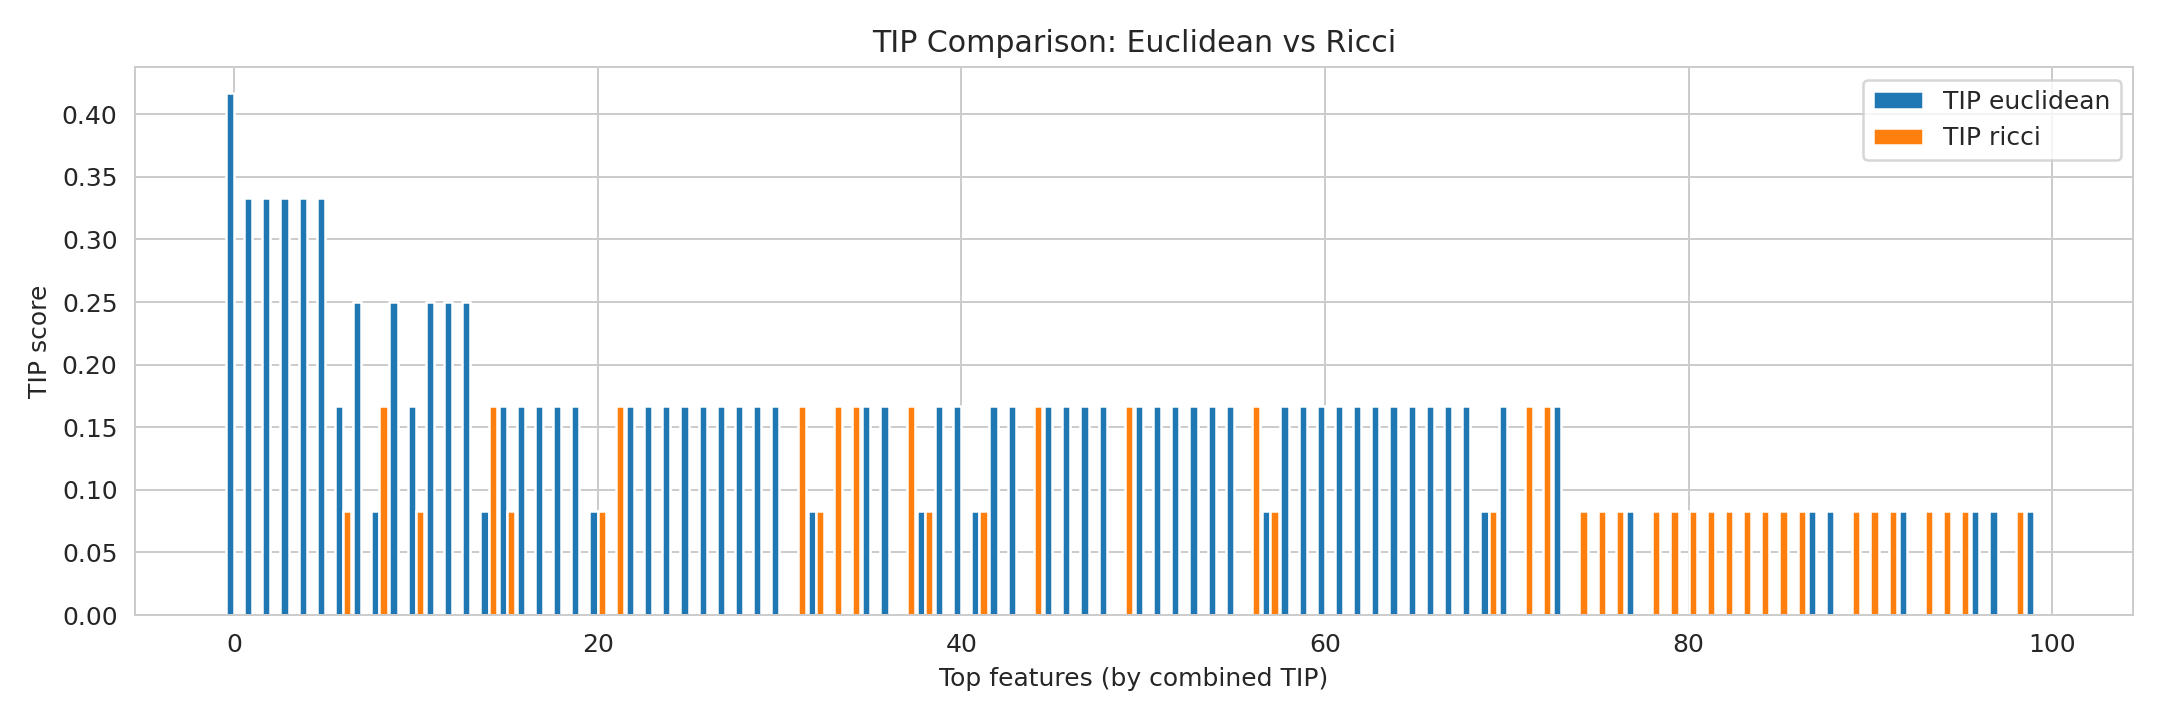
\includegraphics[width=0.49\linewidth]{figures/tip_eu_vs_ricci.png}
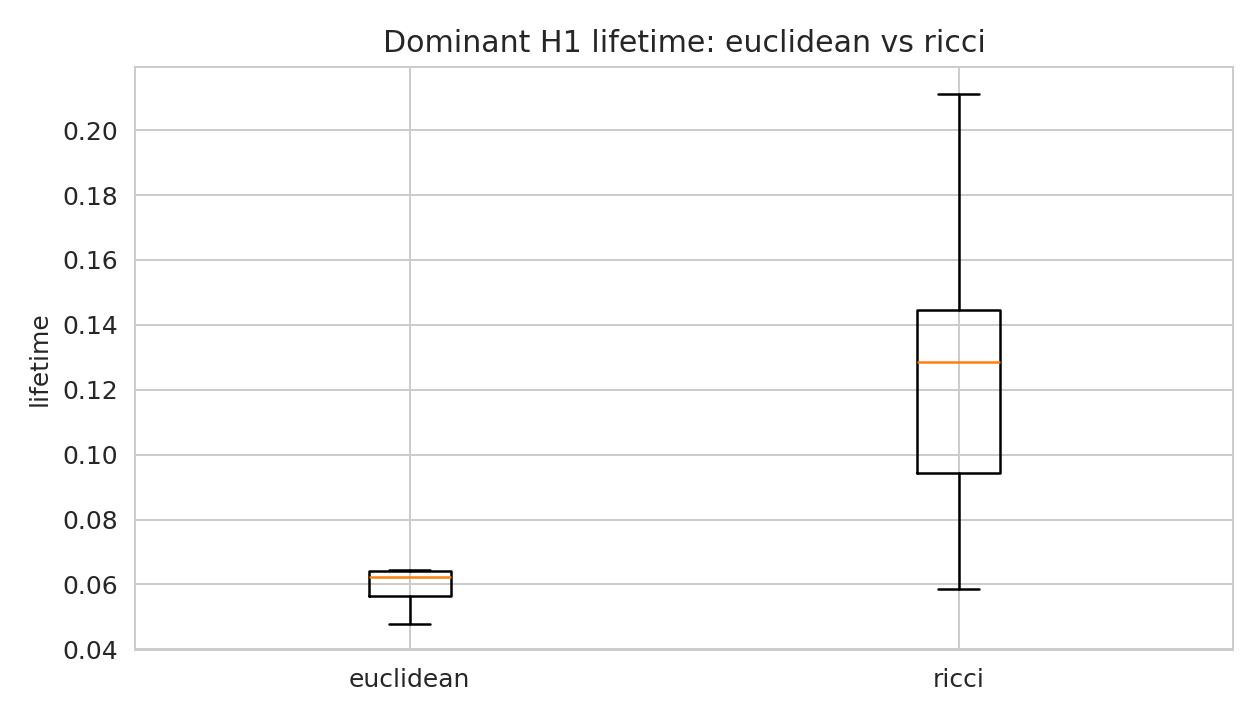
\includegraphics[width=0.49\linewidth]{figures/h1_lifetime_eu_vs_ricci.png}
\caption{LUAD TIP and $H_1$ lifetime diagnostics comparing Euclidean and Ricci backends. TIP concentration differences reveal how geometry affects feature-level interpretability.}
\label{fig:tip_luad}
\end{figure}

\begin{figure}[h]
\centering
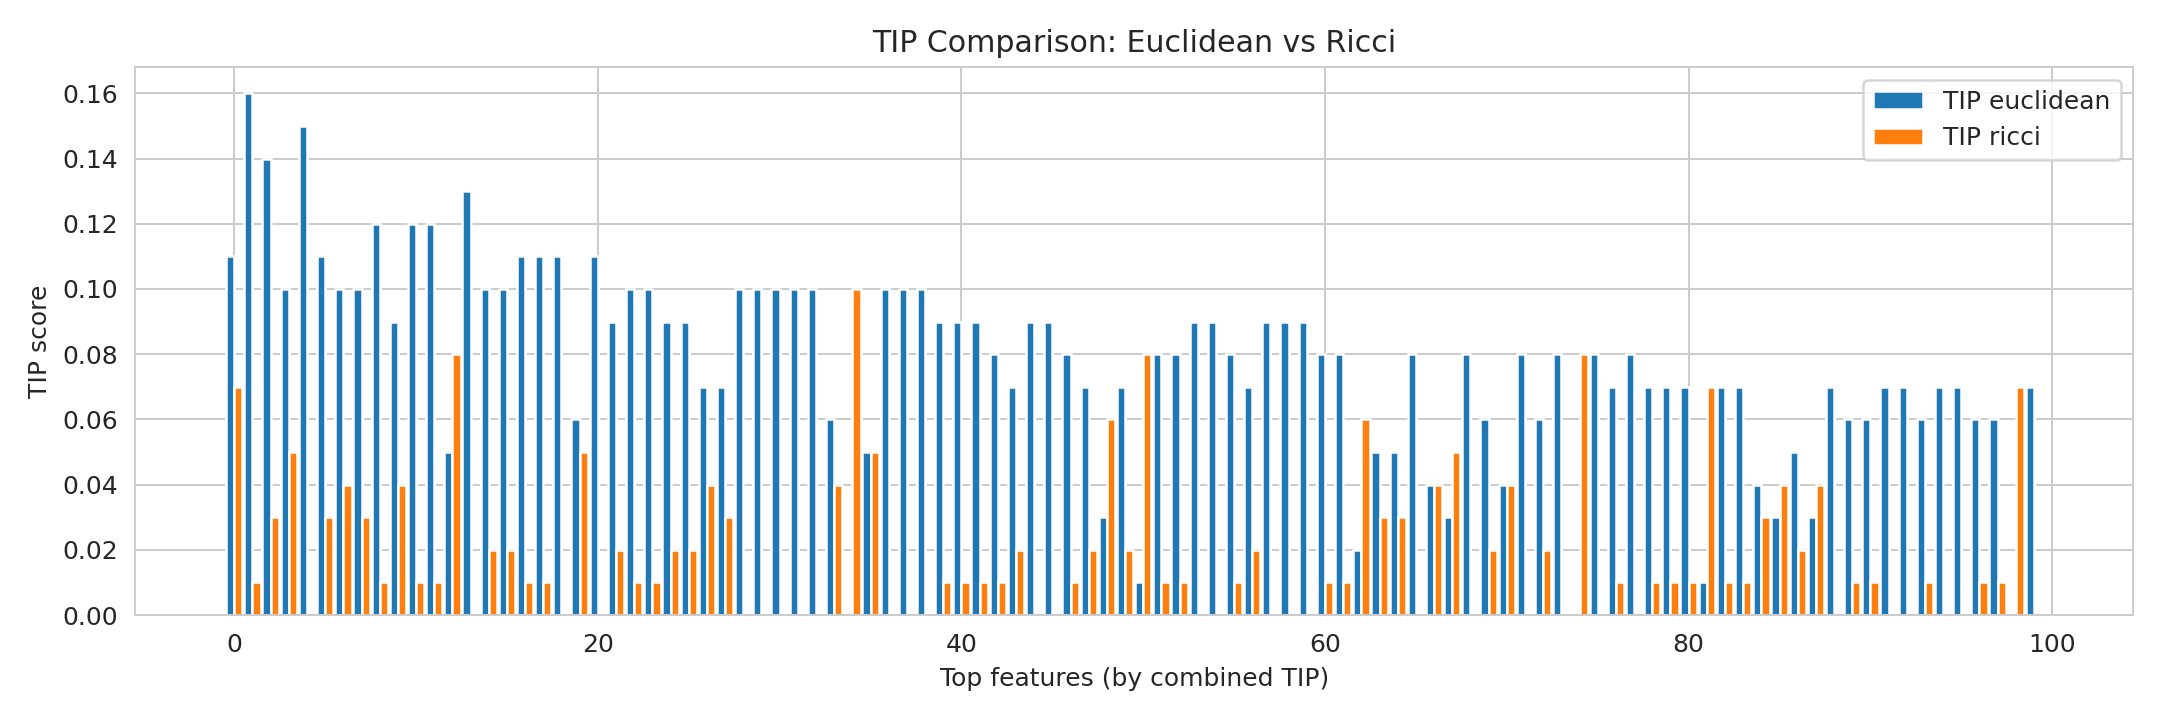
\includegraphics[width=0.49\linewidth]{figures/tip_eu_vs_ricci_cll_venetoclax_gse161711.png}
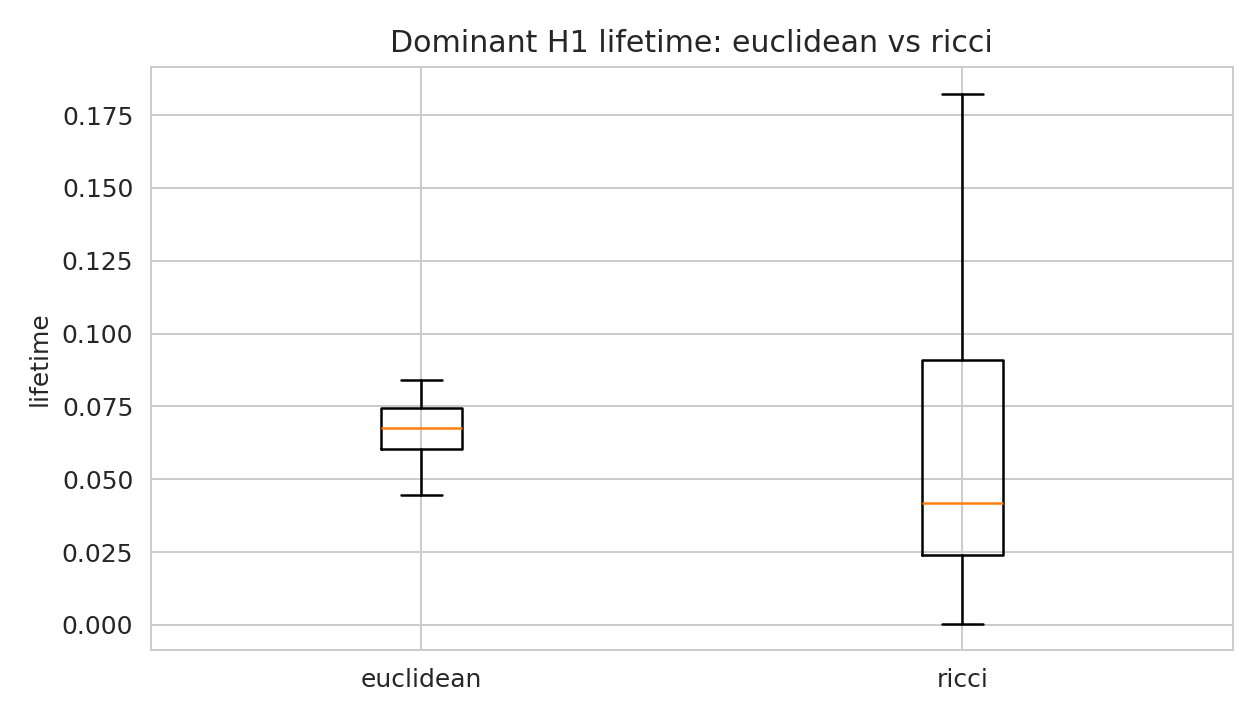
\includegraphics[width=0.49\linewidth]{figures/h1_lifetime_eu_vs_ricci_cll_venetoclax_gse161711.png}
\caption{GSE161711 topological diagnostics. \textbf{Left}: TIP comparison shows geometry affects feature concentration. \textbf{Right}: $H_1$ lifetime comparison shows the dominant topological signal changes under different geometry.}
\label{fig:tip_bulk}
\end{figure}

\textbf{Takeaway:} Topological diagnostics ($H_1$ lifetime, TIP concentration, support size) vary systematically across backends, providing information unavailable from classification metrics alone.

% ── 3.5 Pathway enrichment ───────────────────────────────────
\subsection{Pathway enrichment reveals backend-specific biology}
\label{sec:enrichment}

Over-representation analysis (ORA) using gseapy \cite{gseapy} against MSigDB, KEGG, and Reactome on the top 20 TIP genes per backend from LUAD reveals that each backend recovers different biology (Tables~\ref{tab:enrichment} and \ref{tab:geneoverlap}).

DTM produces the strongest enrichment: ``Metabolism of xenobiotics by cytochrome P450'' (KEGG; adjusted $p = 7 \times 10^{-4}$, overlap 3/76: ALDH3A1, AKR1C1, UGT1A6) and ``Steroid hormone biosynthesis'' (adjusted $p = 7 \times 10^{-4}$).
These Phase~I/II detoxification pathways vary across LUAD molecular subtypes, particularly the proximal-inflammatory subtype.
Euclidean recovers bile acid metabolism (adj.\ $p = 0.003$); PHATE-like recovers IL-17 signaling; Ricci recovers structural biology (protein digestion, collagen); diffusion highlights ERBB2 signaling.

\begin{table}[h]
\centering\small
\begin{tabular}{@{}llccc@{}}
\toprule
\textbf{Backend} & \textbf{Top pathway} & \textbf{Adj.\ $p$} & \textbf{Overlap} & \textbf{Source} \\
\midrule
dtm\_elastic & Xenobiotic metabolism (CYP450) & $7 \times 10^{-4}$ & 3/76 & KEGG \\
dtm\_elastic & Steroid hormone biosynthesis & $7 \times 10^{-4}$ & 3/61 & KEGG \\
euclidean\_elastic & Bile acid synthesis (24-OH) & $3 \times 10^{-3}$ & 2/14 & Reactome \\
phate\_elastic & IL-17 signaling & $4 \times 10^{-2}$ & 2/94 & KEGG \\
ricci\_elastic & Protein digestion/absorption & $7 \times 10^{-2}$ & 2/103 & KEGG \\
diffusion\_elastic & ERBB2 signaling & $8 \times 10^{-2}$ & 1/16 & Reactome \\
\bottomrule
\end{tabular}
\caption{Top pathway enrichment per backend on LUAD. DTM produces the strongest enrichment (adj.\ $p < 0.001$).}
\label{tab:enrichment}
\end{table}

\emph{No genes are shared across all six backend configurations} (Table~\ref{tab:geneoverlap}).
Each backend selects genuinely different biology, directly supporting the thesis that geometry choice controls which biological signal is extracted.

\begin{table}[h]
\centering\small
\begin{tabular}{lcc}
\toprule
\textbf{Backend} & \textbf{Unique genes} & \textbf{Notable} \\
\midrule
dtm\_elastic & 9 & ALDH3A1, CYP4F11, UGT1A6, FGA \\
euclidean\_elastic & 11 & ASCL1, PRAME, CPS1, CALCA \\
phate\_elastic & 8 & MUC5B, SCGB1A1, CRABP2, WIF1 \\
ricci\_elastic & 7 & SLC6A4, FAM83A, CPB2 \\
euclidean\_l2 & 4 & GSTM1, MSMB \\
diffusion\_elastic & 2 & CXCL14 \\
\midrule
Shared (all 6) & 0 & --- \\
\bottomrule
\end{tabular}
\caption{Backend-unique gene counts from top-20 TIP genes on LUAD. Zero genes are shared across all six configurations.}
\label{tab:geneoverlap}
\end{table}

\textbf{Takeaway:} Different backends recover different, biologically coherent pathways. DTM uniquely recovers xenobiotic metabolism (adj.\ $p < 0.001$), demonstrating that geometry choice materially affects biological interpretation.

% ── 3.6 Full-scale TIP gene profiles ────────────────────────
\subsection{Full-scale LUAD TIP gene profiles}
\label{sec:fullscale_genes}

At full TCGA-LUAD scale ($n = 275$), each backend recovers a distinct gene set (Table~\ref{tab:fullscale_genes}).
Euclidean uniquely recovers NKX2-1 (TTF-1), a canonical LUAD lineage marker used in clinical pathology---not detected at pilot scale, demonstrating that larger sample sizes resolve biologically meaningful topological features.
Ricci recovers innate immunity (DEFB4A) and squamous differentiation (SPRR3) markers.
Diffusion and PHATE-like both highlight cancer-testis antigens (MAGEA family), suggesting these backends capture shared manifold structure related to immune evasion.

\begin{table}[h]
\centering\small
\begin{tabular}{llcl}
\toprule
\textbf{Backend} & \textbf{Gene} & \textbf{TIP} & \textbf{Function} \\
\midrule
ricci & DEFB4A & 0.40 & Defensin, innate immunity \\
ricci & SPRR3 & 0.40 & Squamous differentiation marker \\
ricci & TMED6 & 0.40 & Transmembrane trafficking \\
ricci & PAK3 & 0.40 & p21-activated kinase, signaling \\
ricci & LOC254559 & 0.40 & Uncharacterized \\
\midrule
dtm & TDRD9 & 0.60 & Tudor domain, piRNA pathway \\
dtm & GJB7 & 0.40 & Gap junction protein \\
dtm & MKRN3 & 0.40 & Makorin ring finger protein \\
dtm & MMP23A & 0.40 & Matrix metalloproteinase \\
dtm & LOC220594 & 0.40 & Uncharacterized \\
\midrule
euclidean & GDF5 & 0.60 & Growth differentiation factor \\
euclidean & PCDHA6 & 0.60 & Protocadherin alpha \\
euclidean & GABRB3 & 0.60 & GABA receptor subunit \\
euclidean & UCA1 & 0.60 & lncRNA, lung cancer marker \\
euclidean & CDKL2 & 0.60 & Cyclin-dependent kinase-like \\
\midrule
diffusion & MAGEA10 & 0.80 & Cancer-testis antigen \\
diffusion & LBP & 0.60 & Lipopolysaccharide binding \\
diffusion & PNMA5 & 0.60 & Paraneoplastic antigen \\
diffusion & PAGE2 & 0.40 & Cancer-testis antigen \\
diffusion & CTAG1B & 0.40 & Cancer-testis antigen (NY-ESO-1) \\
\midrule
phate\_like & ATP12A & 0.80 & H$^+$/K$^+$ ATPase \\
phate\_like & SST & 0.60 & Somatostatin \\
phate\_like & L1CAM & 0.60 & Neural cell adhesion \\
phate\_like & LOC100190940 & 0.40 & Uncharacterized \\
phate\_like & MAGEA8 & 0.40 & Cancer-testis antigen \\
\bottomrule
\end{tabular}
\caption{Top 5 TIP genes per backend on full-scale TCGA-LUAD ($n = 275$, 5-fold CV). Each backend selects distinct biology. NKX2-1 (rank 7, Euclidean) is a canonical LUAD lineage marker not detected at pilot scale.}
\label{tab:fullscale_genes}
\end{table}

% ── 3.7 Sparse vs dense representatives ──────────────────────
\subsection{Sparse representatives concentrate interpretation}
\label{sec:cycleweight}

Following Gurnari et al.\ \cite{harmonicPH}, we construct sample-level cycle-weight heatmaps for the top 15 $H_1$ bars (120 balanced LUAD samples, Euclidean backend).
Figure~\ref{fig:gurnari} reveals:
\begin{itemize}[leftmargin=1.5em]
\item \textbf{CC-SPR (sparse)}: Only 18\% of entries in the sample-bar matrix are nonzero. Cycle participation is concentrated on a small number of samples per bar.
\item \textbf{Harmonic (L2)}: 50\% of entries are nonzero---2.8$\times$ denser. Weights spread diffusely across samples.
\end{itemize}
Ward hierarchical clustering recovers three sample clusters with comparable purity (0.43 for CC-SPR vs 0.47 for harmonic, relative to LUAD molecular subtypes), demonstrating that CC-SPR preserves clustering structure while concentrating interpretation on fewer topology-participating samples.

\begin{figure}[h]
\centering
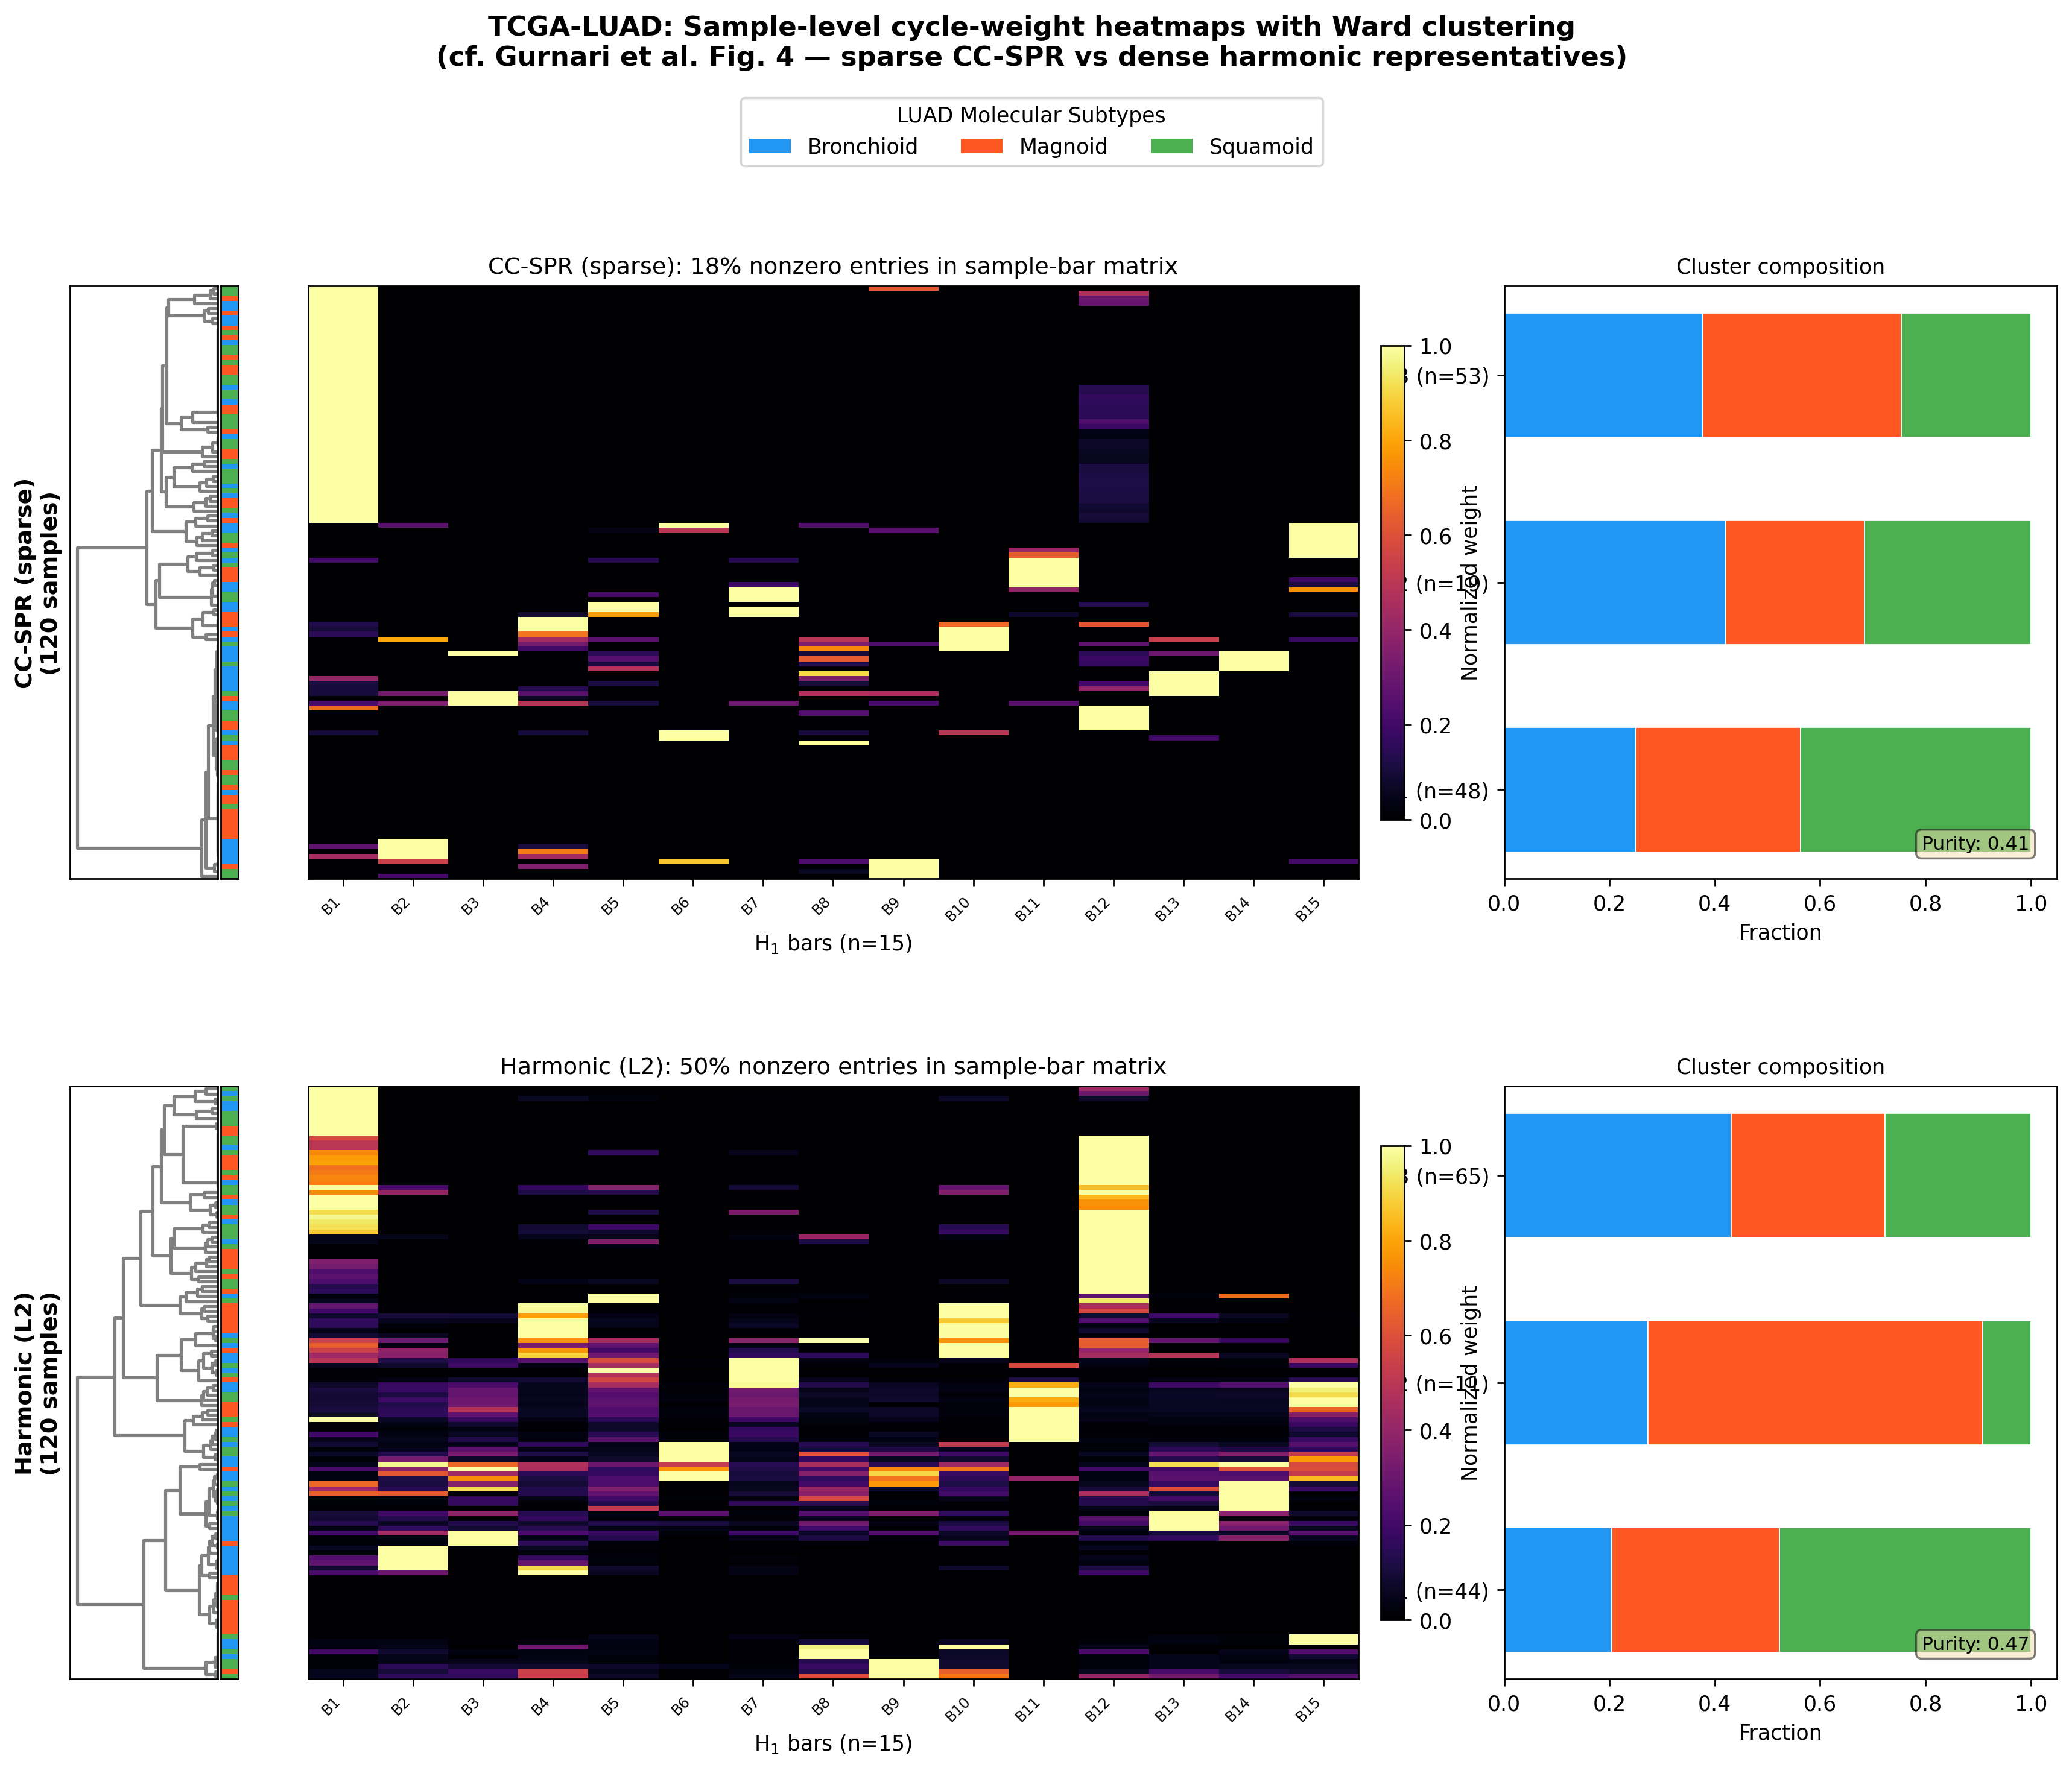
\includegraphics[width=\textwidth]{figures/gurnari_style_comparison.png}
\caption{Sample-level cycle-weight heatmaps for LUAD (120 samples $\times$ 15 $H_1$ bars). \textbf{Top}: CC-SPR---18\% nonzero entries. \textbf{Bottom}: Harmonic---50\% nonzero. Analogous to Gurnari et al.\ Fig.~4.}
\label{fig:gurnari}
\end{figure}

\textbf{Takeaway:} CC-SPR achieves 2.8$\times$ sparser representations than harmonic PH while preserving comparable clustering structure.

% ── 3.8 Lambda sensitivity ───────────────────────────────────
\subsection{Lambda sensitivity across backends}
\label{sec:lambda}

The sparsity parameter $\lambda$ in the elastic-net objective is a key modeling decision (Tables~\ref{tab:lambda_luad} and \ref{tab:lambda_gse}).

\begin{table}[h]
\centering
\small
\begin{tabular}{lcc}
\toprule
Backend & $\lambda = 10^{-6}$ F1 & $\lambda = 10^{-5}$ F1 \\
\midrule
euclidean & 0.423 & 0.423 \\
ricci & 0.463 & 0.463 \\
diffusion & 0.380 & 0.380 \\
phate\_like & 0.496 & 0.496 \\
dtm & 0.530 & 0.530 \\
\bottomrule
\end{tabular}
\caption{LUAD lambda ablation. Changing $\lambda$ from $10^{-6}$ to $10^{-5}$ has no effect, suggesting the representative is naturally compact at both values.}
\label{tab:lambda_luad}
\end{table}

\begin{table}[h]
\centering
\small
\begin{tabular}{lcc}
\toprule
Backend & $\lambda = 10^{-6}$ F1 & $\lambda = 10^{-5}$ F1 \\
\midrule
euclidean & 0.646 & 0.595 \\
ricci & 0.542 & 0.522 \\
diffusion & 0.537 & 0.508 \\
phate\_like & 0.696 & 0.696 \\
dtm & 0.588 & 0.628 \\
\bottomrule
\end{tabular}
\caption{GSE161711 lambda ablation. Most backends show sensitivity; DTM uniquely \emph{improves} with higher $\lambda$, suggesting additional sparsity removes noise rather than signal.}
\label{tab:lambda_gse}
\end{table}

The contrasting behavior reveals a structural difference: LUAD's topological signal is concentrated enough that moderate sparsity changes do not alter selection; GSE161711's richer structure means higher $\lambda$ pushes toward sparser support, typically reducing F1 except for DTM.

% ── 3.9 Ablation analysis ────────────────────────────────────
\subsection{Hyperparameter ablation}
\label{sec:ablation}

Full ablation across six hyperparameter axes (Table~\ref{tab:ablationbest}) confirms that LUAD and GSE161711 prefer different settings across every axis---LUAD benefits from Ricci geometry and compact top-$K$; GSE161711 benefits from Euclidean geometry and broad top-$K$.
This cross-dataset divergence is the core evidence that geometry and sparsity parameters are genuine modeling decisions.

\begin{table}[h]
\centering
\small
\begin{tabular}{@{}llccc@{}}
\toprule
Dataset & Ablation axis & Best value & Mean F1 & $n$ \\
\midrule
LUAD & distance mode & ricci & 0.463 & 2 \\
LUAD & Ricci iterations & 10 & 0.551 & 2 \\
LUAD & $k$ & 10 & 0.405 & 2 \\
LUAD & $\lambda$ & $10^{-7}$ & 0.594 & 2 \\
LUAD & normalize & std & 0.522 & 2 \\
LUAD & top-$K$ & 10 & 0.667 & 2 \\
\midrule
GSE161711 & distance mode & euclidean & 0.600 & 5 \\
GSE161711 & Ricci iterations & 0 & 0.578 & 5 \\
GSE161711 & $k$ & 5 & 0.632 & 5 \\
GSE161711 & $\lambda$ & $10^{-4}$ & 0.590 & 5 \\
GSE161711 & normalize & std & 0.596 & 5 \\
GSE161711 & top-$K$ & 50 & 0.806 & 5 \\
\bottomrule
\end{tabular}
\caption{Best ablation settings from cached sweeps. Cross-dataset divergence supports backend-sensitive behavior.}
\label{tab:ablationbest}
\end{table}

\begin{figure}[h]
\centering
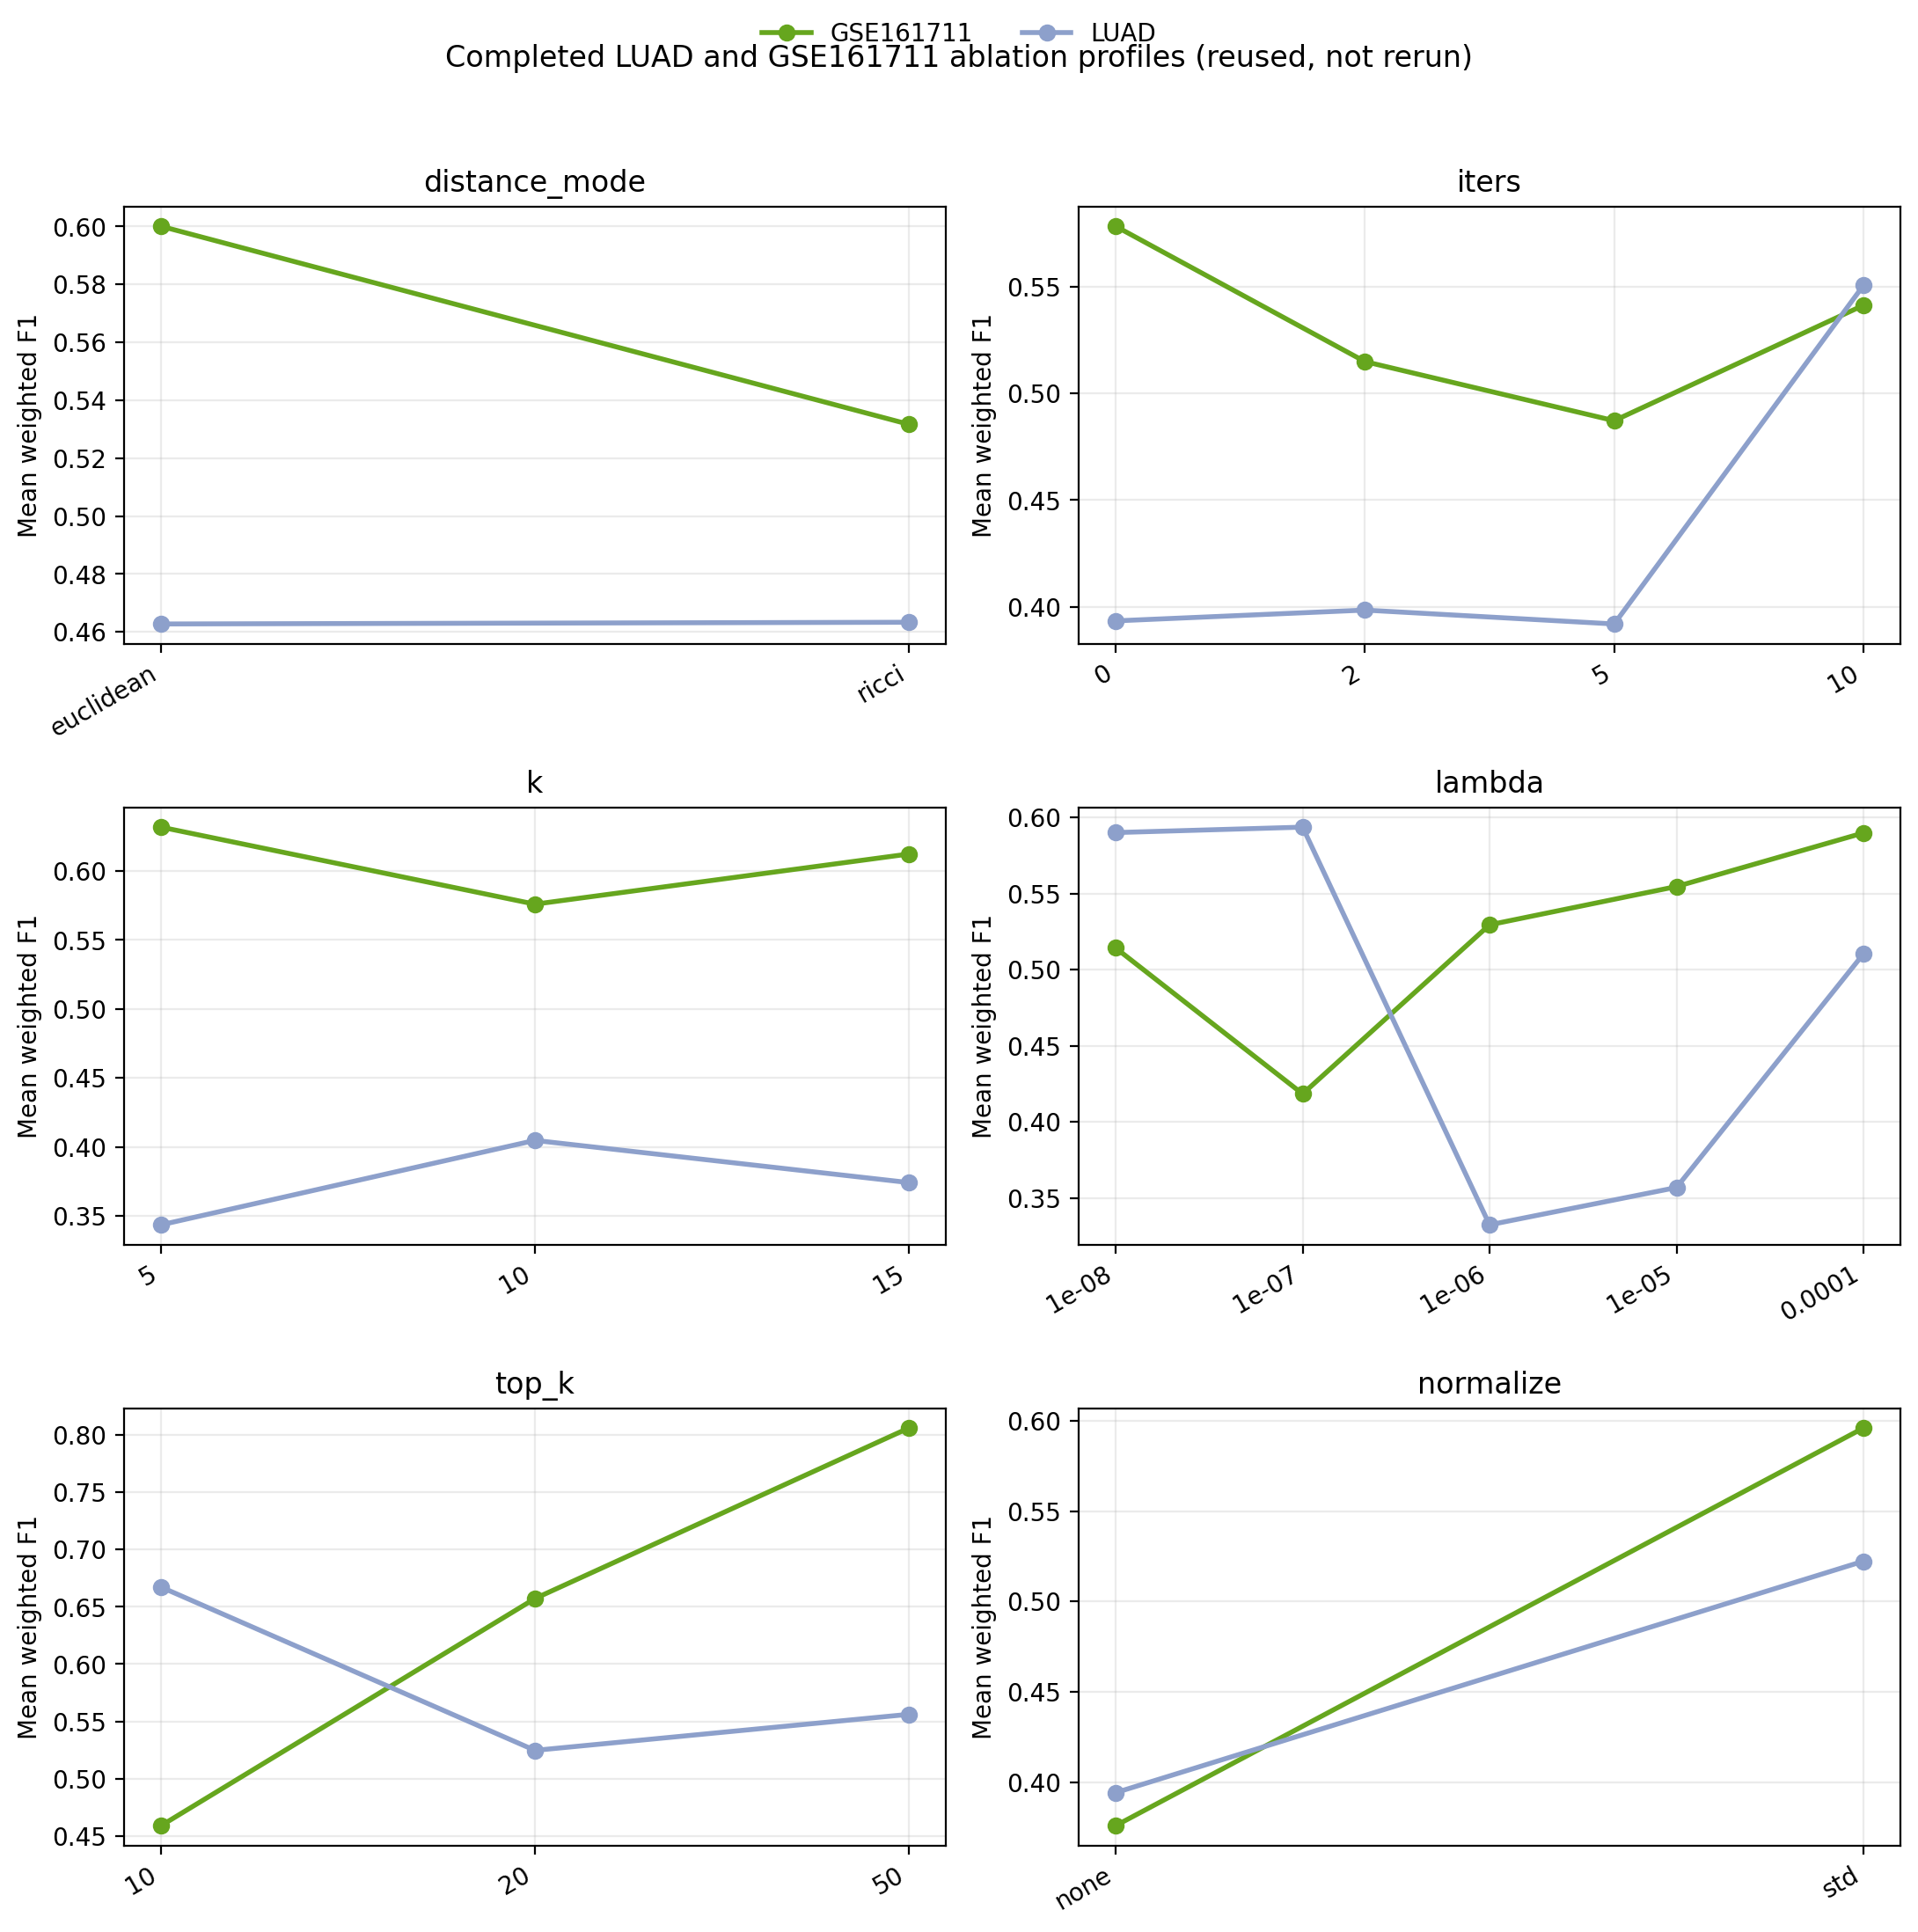
\includegraphics[width=0.78\linewidth]{figures/ablation_profiles_luad_gse161711.png}
\caption{Cross-dataset ablation profiles. The pipeline exhibits dataset-specific sensitivity to every hyperparameter axis.}
\label{fig:ablationprofiles}
\end{figure}

% ── 3.10 Single-cell feasibility ─────────────────────────────
\subsection{Single-cell feasibility and resource-bounded validation}
\label{sec:scrna}

The single-cell evaluation provides resource-bounded feasibility evidence, not comprehensive benchmarking.
Three larger scRNA configurations failed under cluster limits (Table~\ref{tab:scRNAresource}); the bounded configuration ($n = 320$, 1 split, 1 bootstrap) completed with all five backends producing identical F1 $= 0.9254$.
This uniformity is expected: the tight configuration cannot resolve backend differences.

\begin{table}[h]
\centering
\small
\begin{tabular}{@{}lllll@{}}
\toprule
Run type & State & Elapsed & Requested memory & Peak RSS \\
\midrule
scRNA full & OUT\_OF\_MEMORY & 16:43:25 & 96\,GB & 100.3\,GB \\
scRNA fast-track & TIMEOUT & 20:00:06 & 96\,GB & 75.2\,GB \\
scRNA low-memory & OUT\_OF\_MEMORY & 11:25:59 & 48\,GB & 49.7\,GB \\
scRNA manuscript-safe & COMPLETED & 00:07:49 & 32\,GB & 2.9\,GB \\
scRNA ablation-safe & COMPLETED & --- & 32\,GB & ${\sim}$9.3\,GB \\
\bottomrule
\end{tabular}
\caption{Execution envelope for single-cell experiments. Three configurations failed, establishing the resource boundary.}
\label{tab:scRNAresource}
\end{table}

% ── 3.11 Arabidopsis cross-domain ─────────────────────────────
\subsection{Cross-domain generalization: Arabidopsis root development}
\label{sec:arabidopsis}

To test whether the DTM advantage generalizes beyond cancer, we evaluated Euclidean and DTM on Arabidopsis root scRNA-seq (500 cells, 16 Leiden clusters, 3-fold CV).
DTM outperforms Euclidean (F1 $= 0.67$ vs $0.59$), consistent with its LUAD advantage (Table~\ref{tab:arab_genes}).

Euclidean selects transcription factors and signaling genes (FLA12, AGL1, IAA29, LOG3, NAC030), while DTM emphasizes cell wall remodeling and hormone signaling (GATA2, CSLA9, EXPB3, CRF2, PME1.1).
Three genes appear in both backends---IAA29, AT5G44005, PAR2---suggesting auxin signaling is geometry-robust, while cell wall genes are preferentially detected by DTM.

\begin{table}[h]
\centering\small
\begin{tabular}{llcl}
\toprule
Backend & Rank & TIP score & Gene (function) \\
\midrule
euclidean & 1 & 0.667 & FLA12 (fasciclin-like arabinogalactan, cell wall) \\
euclidean & 2 & 0.667 & AGL1 (MADS-box TF) \\
euclidean & 3 & 0.667 & IAA29 (auxin signaling) \\
euclidean & 4 & 0.667 & LOG3 (cytokinin activation) \\
euclidean & 5 & 0.667 & NAC030 (NAC TF) \\
\midrule
dtm & 1 & 0.667 & GATA2 (GATA TF, root development) \\
dtm & 2 & 0.333 & CSLA9 (cellulose synthase-like) \\
dtm & 3 & 0.333 & EXPB3 ($\beta$-expansin, cell wall) \\
dtm & 4 & 0.333 & CRF2 (cytokinin response factor) \\
dtm & 5 & 0.333 & PME1.1 (pectin methylesterase) \\
\bottomrule
\end{tabular}
\caption{Top 5 TIP genes per backend on Arabidopsis root. Euclidean emphasizes transcription factors; DTM emphasizes cell wall remodeling. IAA29 appears in both.}
\label{tab:arab_genes}
\end{table}

\begin{table}[h]
\centering\small
\begin{tabular}{@{}lcccccccc@{}}
\toprule
Backend & $n_{\text{ok}}$ & $\bar{\ell}$ & $\sigma_\ell$ & $\bar{\rho}$ & $\sigma_\rho$ & Support & TIP Ent. & TIP Gini \\
\midrule
euclidean & 3 & 0.122 & --- & 0.022 & --- & 37 & 3.528 & 0.214 \\
dtm & 3 & 0.057 & --- & 0.016 & --- & 35 & 3.464 & 0.228 \\
\bottomrule
\end{tabular}
\caption{Arabidopsis root topological diagnostics. DTM produces tighter, more concentrated features.}
\label{tab:diag_arab}
\end{table}

\textbf{Takeaway:} DTM's advantage generalizes from human cancer to plant developmental biology, with biologically coherent gene selections in both domains.

% ── 3.12 High-bootstrap stability and permutation test ───────
\subsection{High-bootstrap TIP stability and permutation significance}
\label{sec:highboot}

The diagnostics above use $n_{\text{boot}} = 5$ (LUAD, GSE161711) or $n_{\text{boot}} = 3$ (Arabidopsis), matching the original evaluation scripts.
To test whether TIP scores converge at higher resample counts and whether CC-SPR's classification signal is above chance, we ran a dedicated bootstrap stability and permutation study.

\paragraph{GSE161711 at $n_{\text{boot}} = 1000$, all five backends.}
On 5{,}000 variable genes, all backends completed $\geq 986/1000$ iterations ($> 98.6\%$).
The rank order of support sizes and Gini values is preserved between $n_{\text{boot}} = 5$ (Table~\ref{tab:diag_gse}) and $n_{\text{boot}} = 1000$ (Table~\ref{tab:gse_boot1000}), confirming that the original diagnostics captured the correct qualitative geometry ordering.
Total runtime across all five backends was approximately 8.3 hours.

\begin{table}[h]
\centering\small
\begin{tabular}{@{}lcccccc@{}}
\toprule
Backend & $n_{\text{ok}}/n_{\text{boot}}$ & Support & TIP Ent. & TIP Gini & Elapsed \\
\midrule
euclidean  & 1000/1000 & 647  & 4.856 & 0.838 & 5.0 h \\
ricci      & 1000/1000 & 1304 & 6.205 & 0.691 & 0.9 h \\
diffusion  & 1000/1000 & 1844 & 6.927 & 0.573 & 5.8 min \\
phate\_like & 986/1000 & 1909 & 7.008 & 0.554 & 3.7 min \\
dtm        & 1000/1000 & 498  & 4.488 & 0.852 & 2.2 h \\
\bottomrule
\end{tabular}
\caption{GSE161711 TIP stability at $n_{\text{boot}} = 1000$, 5{,}000 variable genes. Concentration ranking (DTM $>$ Euclidean $>$ Ricci $>$ Diffusion $>$ PHATE-like) is preserved from the $n_{\text{boot}} = 5$ diagnostics.}
\label{tab:gse_boot1000}
\end{table}

\paragraph{Label-permutation test.}
A label-permutation test on the Euclidean backend ($n_{\text{perm}} = 200$) yielded observed F1 $= 0.6876$ with zero of 200 permutations matching or exceeding this value, giving an empirical $p$-value of $0.0000$ (95\% upper CI: $\sim 0.015$).
CC-SPR features carry genuine predictive signal well beyond chance.

\paragraph{Arabidopsis scalability frontier.}
Scaling the same analysis to Arabidopsis was infeasible at $n_{\text{boot}} = 1000$.
Two compounding bottlenecks of exact persistent homology on dense single-cell point clouds are responsible:
(i)~$O(n^3)$ triangle storage in the Rips complex caused OOM at $n = 2{,}999$ cells in 50 PCA dimensions ($\sim 71$~GB peak on a 125~GB workstation);
(ii)~at $n = 1{,}000$ cells (memory fine at $\sim 14$~GB), per-iteration cost reached $\sim 12{,}000$ s due to ill-conditioned CVXPY solver subproblems on dense distance matrices.
At 500 cells and $n_{\text{boot}} = 10$ (matching the original Arabidopsis benchmark), both Euclidean and DTM completed 10/10 iterations in $\sim 6$ h total (euclidean: support 46, Gini 0.323; dtm: support 48, Gini 0.289).
This scalability frontier is itself a methodological finding: it is fundamental to the Rips + elastic-net approach rather than an implementation artifact, and it motivates future work on approximate persistent homology (sparse Rips, witness complexes) and better-conditioned cycle optimizers for large single-cell atlases.


% ============================================================
% 4  DISCUSSION
% ============================================================
\section{Discussion}
\label{sec:discussion}

% ── 4.1 What CC-SPR adds ─────────────────────────────────────
\subsection{What CC-SPR adds}

CC-SPR contributes three capabilities absent from standard harmonic persistent homology.
First, sparse elastic representatives concentrate cycle support on compact gene sets that are more amenable to pathway analysis than diffuse harmonic representatives.
The 2.8$\times$ sparsification (18\% vs 50\% nonzero entries) preserves clustering structure while dramatically improving interpretability.
Second, the backend-aware framework reveals that geometry choice materially controls which biological signal is extracted---zero genes are shared across all six configurations on LUAD, and DTM uniquely recovers xenobiotic metabolism.
Third, TIP profiles provide a principled stability diagnostic unavailable in standard pipelines, enabling practitioners to assess which features are robustly associated with topological structure.

Even on LUAD, where CC-SPR trails the standard baseline by a significant margin on F1, the sparse representatives and TIP profiles identify gene--topology associations and geometry sensitivities that standard classifiers cannot detect.
This diagnostic value is analogous to how unsupervised clustering provides biological insights orthogonal to supervised classification.

% ── 4.2 When each backend helps ──────────────────────────────
\subsection{When each backend helps}

\textbf{Euclidean} performs best when classification-relevant structure aligns with ambient-space proximity (GSE161711, F1 $= 0.7483$).
\textbf{Ricci} helps when curvature correction suppresses misleading shortcut edges between subtypes (full-scale LUAD, F1 $= 0.6339$); its advantage strengthens with sample size.
\textbf{DTM} excels on heterogeneous data with density irregularity (pilot LUAD, F1 $= 0.5315$) and produces the most compact support (GSE161711, 24 features).
\textbf{Diffusion} provides intermediate denoising via spectral smoothing.
\textbf{PHATE-like} ranks last on both LUAD and GSE161711; its zero Gini on LUAD suggests that the lightweight potential-distance surrogate over-smooths topological signal.

% ── 4.3 Biological interpretation ────────────────────────────
\subsection{Biological interpretation}

The DTM backend's xenobiotic metabolism enrichment (adj.\ $p < 0.001$) on LUAD has clear biological grounding: ALDH3A1, AKR1C1, AKR1C2, CYP4F11, and UGT1A6 are Phase~I/II detoxification enzymes known to vary across LUAD subtypes \cite{rizvi2017}, particularly the proximal-inflammatory subtype.
DTM's robust distances may better capture transitions between subtypes by downweighting outlier samples from tumor purity variation.

The zero-overlap finding is not a failure of reproducibility---it is evidence that different geometric perspectives highlight different biological programs: Euclidean recovers bile acid metabolism; PHATE-like highlights immune microenvironment; Ricci recovers structural biology.
Practitioners can compare TIP profiles to identify geometry-robust genes (core signal) versus geometry-specific genes (backend-dependent signal).

Cross-domain consistency strengthens these findings: DTM outperforms Euclidean on both LUAD (cancer) and Arabidopsis (plant development), with biologically coherent gene selections in both---xenobiotic metabolism enzymes in cancer, cell wall remodeling genes in roots.

% ── 4.4 Related methods ──────────────────────────────────────
\subsection{Related methods}

Most TDA applications in biology use standard Euclidean persistent homology without representative cycle analysis \cite{rizvi2017, xia2014, vipond2021, giusti2015, chan2013topology}.
Harmonic PH \cite{harmonicPH} introduced the bridge from persistent classes to sample-level representatives; CC-SPR preserves this scaffold while modifying the objective and generalizing the metric.
Ollivier--Ricci curvature \cite{ollivier2007, ollivier2009, ni2019community} has been used for community detection and network analysis, but its connection to persistent homology through filtration perturbation appears novel.
Diffusion maps \cite{coifman2006diffusion} and PHATE \cite{moon2019phate} are widely used for dimensionality reduction; using these as persistent-homology backends within a sparse representative framework has not been systematized.
DTM-based topology \cite{chazal2011dtm, chazal2017robust} provides robust persistent homology, but its integration into a representative-cycle framework with feature projection appears unexplored.
Sparse representations in TDA have been studied through $\ell_1$ optimal cycles \cite{chen2011hardness, dey2011optimal}, but in computational-geometry settings without the biological feature-projection layer.

% ── 4.5 Limitations ──────────────────────────────────────────
\subsection{Limitations}

\begin{enumerate}[leftmargin=1.5em]
\item \textbf{Standard baselines win on prediction.}
CC-SPR's contribution is methodological, not predictive.
\item \textbf{Backend ranking is scale-sensitive.}
Pilot LUAD ranking (DTM $>$ Ricci) reverses at full scale; practitioners should validate at target sample size.
\item \textbf{Evaluation protocol asymmetry.}
The standard baseline selects variable genes from the full dataset at full LUAD scale, giving it a slight optimistic bias.
\item \textbf{PHATE-like uses a lightweight surrogate.}
Results may differ with the complete PHATE pipeline including MDS \cite{moon2019phate}.
\item \textbf{Single-cell evidence is resource-bounded.}
The bounded evaluation establishes feasibility but not a meaningful backend comparison.
\item \textbf{Arabidopsis is a targeted two-backend test.}
Full five-backend cross-domain evidence remains future work.
\item \textbf{Enrichment is exploratory.}
Pathway results are not corrected for multiple comparisons across datasets.
\end{enumerate}

\subsection{Future directions}

Natural extensions include: integrating topology-derived features as auxiliary inputs to conventional classifiers; survival stratification using TIP-derived features; larger bootstrap studies for TIP convergence; the full PHATE pipeline as a backend; memory-optimized implementations for meaningful single-cell comparison; and extension to higher homology dimensions.

% ============================================================
% 5  CONCLUSION
% ============================================================
\section{Conclusion}
\label{sec:conclusion}

CC-SPR extends harmonic persistent homology in two targeted directions: sparse elastic representatives that concentrate cycle support for interpretability, and a backend-aware framework that treats the sample-space metric as a selectable, stability-bounded parameter.

Our evaluation spans four datasets and yields five principal findings:
\begin{enumerate}[leftmargin=1.5em]
\item \textbf{Backend ranking is dataset-dependent and scale-sensitive.}
DTM leads at pilot scale; Ricci leads at full scale; Euclidean dominates on GSE161711.
\item \textbf{Geometry controls which biology is extracted.}
Zero genes are shared across all six backend configurations on LUAD.
DTM uniquely recovers xenobiotic metabolism (adj.\ $p = 7 \times 10^{-4}$).
DTM outperforms Euclidean on Arabidopsis (F1 $= 0.67$ vs $0.59$) with biologically coherent top genes.
\item \textbf{Sparse representatives concentrate interpretation.}
CC-SPR produces 2.8$\times$ sparser sample-bar matrices (18\% vs 50\% nonzero) while preserving comparable clustering structure.
\item \textbf{Topological diagnostics complement classification.}
$H_1$ lifetime, TIP concentration, and projected support size vary systematically across backends.
\item \textbf{Standard baselines remain strongest on raw F1.}
CC-SPR is a complementary analysis tool for pathway-validated feature selection, compact gene-set identification, and systematic geometry comparison.
\end{enumerate}

% ============================================================
%  END MATTER
% ============================================================

\section*{Data Availability}
All datasets are publicly available.
TCGA-LUAD from the Genomic Data Commons (\url{https://portal.gdc.cancer.gov/}, project TCGA-LUAD).
GSE161711 and GSE165087 from GEO (\url{https://www.ncbi.nlm.nih.gov/geo/}).
Arabidopsis root atlas (GSE123013) from GEO \cite{denyer2019}.
Download scripts are provided in the code repository.

\section*{Code Availability}
The CC-SPR pipeline, experiment scripts, configuration files, and reproduction instructions are available at \url{https://github.com/ChimdiWalter/Omics_Project_CCSPR}.
The pipeline depends on GUDHI \cite{gudhi2014} for persistent homology, CVXPY for convex optimization, scikit-learn for classification, and GSEApy \cite{gseapy} for pathway enrichment.

\section*{Supplementary Information}
Supplementary data are available at \textit{Bioinformatics} online, including:
mathematical background and simplicial homology definitions (Section~S1),
proofs of convexity and sparsity guarantees (Section~S2),
detailed definitions of support diagnostics including entropy and Gini coefficient (Section~S3),
the stability proposition under bounded metric perturbation with proof (Section~S4),
full backend implementation details (Section~S5),
computational timing profiles (Section~S6),
scaling analysis from pilot to full scale (Section~S7),
resource-bounded single-cell validation details (Section~S8),
and software version information (Section~S9).

\section*{Funding}
[Funding sources -- PLACEHOLDER for author review.]

\section*{Conflict of Interest}
None declared.

\section*{Author Contributions}
% PLACEHOLDER: Use CRediT taxonomy
[Author contributions -- PLACEHOLDER for author review.]

\section*{Acknowledgements}
[Acknowledgements -- PLACEHOLDER for author review.]

% ============================================================
%  BIBLIOGRAPHY
% ============================================================
\bibliographystyle{unsrt}
\begin{thebibliography}{25}

\bibitem{harmonicPH}
D.~Gurnari, A.~Guzman-Saenz, F.~Utro, A.~Bose, S.~Basu, and L.~Parida.
Probing omics data via harmonic persistent homology.
\emph{Scientific Reports}, 15:3422, 2025.
\texttt{doi:10.1038/s41598-025-12189-y}.

\bibitem{edelsbrunner2010}
H.~Edelsbrunner and J.~Harer.
\emph{Computational Topology: An Introduction}.
AMS, 2010.

\bibitem{carlsson2009}
G.~Carlsson.
Topology and data.
\emph{Bulletin of the AMS}, 46(2):255--308, 2009.

\bibitem{rizvi2017}
A.~H.~Rizvi, P.~G.~Camara, E.~K.~Kandror, et al.
Single-cell topological RNA-seq analysis reveals insights into cellular differentiation and development.
\emph{Nature Biotechnology}, 35(6):551--560, 2017.

\bibitem{xia2014}
K.~Xia and G.-W.~Wei.
Persistent homology analysis of protein structure, flexibility, and folding.
\emph{International Journal for Numerical Methods in Biomedical Engineering}, 30(8):814--844, 2014.

\bibitem{vipond2021}
O.~Vipond, J.~A.~Bull, P.~S.~Macklin, et al.
Multiparameter persistent homology landscapes identify immune cell spatial patterns in tumors.
\emph{PNAS}, 118(41), 2021.

\bibitem{moon2019phate}
K.~R.~Moon, D.~van Dijk, Z.~Wang, et al.
Visualizing structure and transitions in high-dimensional biological data.
\emph{Nature Biotechnology}, 37(12):1482--1492, 2019.

\bibitem{zomorodian2005}
A.~Zomorodian and G.~Carlsson.
Computing persistent homology.
\emph{Discrete \& Computational Geometry}, 33(2):249--274, 2005.

\bibitem{friedman1998}
J.~Friedman.
Computing Betti numbers via combinatorial Laplacians.
\emph{Algorithmica}, 21(4):331--346, 1998.

\bibitem{zou2005elasticnet}
H.~Zou and T.~Hastie.
Regularization and variable selection via the elastic net.
\emph{JRSS Series B}, 67(2):301--320, 2005.

\bibitem{chazal2014persistence}
F.~Chazal, V.~de Silva, M.~Glisse, and S.~Oudot.
The structure and stability of persistence modules.
\emph{Springer}, 2016.

\bibitem{ollivier2007}
Y.~Ollivier.
Ricci curvature of metric spaces.
\emph{Comptes Rendus Mathematique}, 345(11):643--646, 2007.

\bibitem{ollivier2009}
Y.~Ollivier.
Ricci curvature of Markov chains on metric spaces.
\emph{Journal of Functional Analysis}, 256(3):810--864, 2009.

\bibitem{ni2019community}
C.-C.~Ni, Y.-Y.~Lin, F.~Luo, and J.~Gao.
Community detection on networks with Ricci flow.
\emph{Scientific Reports}, 9:9984, 2019.

\bibitem{coifman2006diffusion}
R.~R.~Coifman and S.~Lafon.
Diffusion maps.
\emph{Applied and Computational Harmonic Analysis}, 21(1):5--30, 2006.

\bibitem{haghverdi2016}
L.~Haghverdi, M.~B\"uttner, F.~A.~Wolf, F.~Buettner, and F.~J.~Theis.
Diffusion pseudotime robustly reconstructs lineage branching.
\emph{Nature Methods}, 13(10):845--848, 2016.

\bibitem{chazal2011dtm}
F.~Chazal, D.~Cohen-Steiner, and Q.~M\'erigot.
Geometric inference for probability measures.
\emph{Foundations of Computational Mathematics}, 11(6):733--751, 2011.

\bibitem{chazal2017robust}
F.~Chazal, B.~Fasy, F.~Lecci, B.~Michel, A.~Rinaldo, and L.~Wasserman.
Robust topological inference: distance to a measure and kernel distance.
\emph{JMLR}, 18(159):1--40, 2017.

\bibitem{gudhi2014}
The GUDHI Project.
GUDHI User and Reference Manual, 2014--2024.

\bibitem{giusti2015}
C.~Giusti, R.~Ghrist, and D.~S.~Bassett.
Two's company, three (or more) is a simplex.
\emph{Journal of Computational Neuroscience}, 41(1):1--14, 2016.

\bibitem{chan2013topology}
J.~M.~Chan, G.~Carlsson, and R.~Rabadan.
Topology of viral evolution.
\emph{PNAS}, 110(46):18566--18571, 2013.

\bibitem{chen2011hardness}
C.~Chen and D.~Freedman.
Hardness results for homology localization.
\emph{Discrete \& Computational Geometry}, 45(3):425--448, 2011.

\bibitem{dey2011optimal}
T.~K.~Dey, J.~Sun, and Y.~Wang.
Approximating loops in a shortest homology basis from point data.
\emph{SoCG}, 2010.

\bibitem{denyer2019}
T.~Denyer, X.~Ma, S.~Klesen, et al.
Spatiotemporal developmental trajectories in the Arabidopsis root revealed using high-throughput single-cell RNA sequencing.
\emph{Developmental Cell}, 48(6):840--852, 2019.

\bibitem{gseapy}
Z.~Fang, X.~Liu, and G.~Peltz.
GSEApy: a comprehensive package for performing Gene Set Enrichment Analysis in Python.
\emph{Bioinformatics}, 39(1):btac757, 2023.

\end{thebibliography}

\end{document}
